%\documentclass{sig-alternate-05-2015}
\documentclass{llncs}
\usepackage{makeidx}
\usepackage{tabularx,colortbl}
\usepackage[dvipsnames]{xcolor}
\usepackage{flushend}
\usepackage{cite}
\usepackage{amsmath}
%\usepackage{amsthm}
\usepackage{amssymb}
\usepackage{epsfig}
\usepackage{stmaryrd}
\usepackage{url}
\usepackage{multirow}
\usepackage{latexsym}
\usepackage{graphics}
\usepackage{graphicx}
\usepackage{enumitem}
\usepackage{comment}
\usepackage{longtable}
\usepackage{supertabular}
\usepackage{times}
\usepackage{listings}
\usepackage{subfigure}
\usepackage{color}
\usepackage{balance}
\usepackage{xspace}
\usepackage[ruled, vlined, linesnumbered]{algorithm2e}
\usepackage[autostyle]{csquotes}
\usepackage[]{algorithm2e}
%\usepackage[font=large]{caption}



%\theoremstyle{Definition}
%\newtheorem{definition}{Definition}
%%%
%\theoremstyle{Theorem}
%\newtheorem{theorem}{Theorem}


%\newcommand{\definition}{\noindent \textbf{Definition} \citation{}}
%\newcommand{\theorem}{\noindent \textbf{Theorem} \citation{}}
%\newcommand{\lemma}{\noindent \textbf{Lemma} \citation{}}

%\newdef{lemma}{Lemma}
%\newdef{definition}{Definition}
%\newdef{theorem}{Theorem}
%\newdef{corollary}{Corollary}
%\newdef{note}{Note}
%\newdef{axiom}{Axiom}
\newcommand{\mkeyword}[1]{\mbox{\texttt{#1}}}
\DeclareMathOperator{\kuop}{uop}
\DeclareMathOperator{\kbop}{bop}
\DeclareMathOperator{\kite}{ite}
\DeclareMathOperator{\kpre}{pre}
\DeclareMathOperator{\dom}{dom}
\DeclareMathOperator{\ktrue}{true}
\DeclareMathOperator{\kfalse}{false}
\DeclareMathOperator{\kselect}{select}
\DeclareMathOperator{\ran}{range}
\newcommand{\lbb}{[\![}
\newcommand{\rbb}{]\!]}
\newcommand{\expr}{\phi}
\newcommand{\exprS}{\Phi}
\newcommand{\mats}[1]{\textcolor{red}{#1}}
\newcommand{\janet}[1]{\textcolor{blue}{#1}}
\newcommand{\darren}[1]{\textcolor{green}{#1}}
\newcommand{\danielle}[1]{\textcolor{orange}{#1}}

\sloppypar



\begin{document}

\definecolor{gold}{rgb}{0.90,.66,0}
\definecolor{dgreen}{rgb}{0,0.6,0}
\newcommand{\stateequiv}{\equiv_{s}}
\newcommand{\traceequiv}{\equiv_{\sigma}}
\newcommand{\ta}{\text{TA}}
\newcommand{\cta}{\text{TA$_{C}$}}
\newcommand{\tta}{\text{TA$_{T}$}}
\newcommand{\ucalg}{\texttt{\small{IVC\_UC}}}
\newcommand{\ucbfalg}{\texttt{\small{IVC\_UCBF}}}


\title{The Safety Annex for the Architecture Analysis and Design Language}
%
\author{Danielle Stewart\inst{1}
\and Jing (Janet) Liu\inst{2}
\and Michael W. Whalen\inst{1}
\and Darren Cofer\inst{2}
\and Mats Heimdahl\inst{1}
\and Michael Peterson\inst{3}}
\institute{University of Minnesota\\Department of Computer
Science and Engineering\\
\email{dkstewar, whalen, heimdahl}@cs.umn.edu
\and
Collins Aerospace\\
%Advanced Technology Center
Trusted Systems - Engineering and Technology
\\
\email{Jing.Liu, Darren.Cofer}@collins.com
\and
Collins Aerospace\\
%Commercial Systems 
Flight Controls Safety Engineering - Avionics\\
\email{Michael.Peterson}@collins.com
}
\maketitle

\begin{abstract}
%Mats' abstract
Model-based development techniques are increasingly being used in the development of critical systems software. Leveraging the artifacts from model based development in the safety analysis process would be highly desirable to provide accurate analysis and enable cost savings. In particular, architectural and behavioral models provide rich information about the system's operation. In this paper we describe an extension 
to the Architecture Analysis and Design Language (AADL) developed to allow a rich modeling of a system under failure conditions. This \emph{Safety Annex} allows the independent modeling of component failure modes and allows safety engineers to weave various types of faults into the nominal system model. 
The accompanying tool support allows investigation of the propagation of errors from their source to their effect on top level safety properties without the need to add separate propagation specifications; 
it  also supports describing dependent faults that are not captured through the behavioral models, 
e.g., failures correlated due to the physical structure of the system.
We describe the Safety Annex, illustrate its use with a representative example, and discuss and demonstrate the tool support enabling an analyst to investigate the system behavior under failure conditions.	
	

\end{abstract}

\keywords{Model-based systems engineering, fault analysis, safety engineering}

\section{Introduction}
\label{sec:intro}

Risk and safety analyses are important activities used to ensure that critical systems operate in an expected way. From nuclear power plants and airplanes to heart monitors and automobiles, critical systems are ubiquitous in our society. These systems are required to operate safely under nominal and faulty conditions. Guaranteeing that system safety properties hold in the presence of faults is an important aspect of critical systems development and falls under the discipline of safety analysis. Safety analysis produces various safety related artifacts that are used during development and certification of critical systems~\cite{SAE:ARP4761,SAE:ARP4754A}. Examples include {\em minimal cut sets} -- the minimal sets of faults that may violate a safety property and {\em fault trees} -- the Boolean formula whose literals are minimal cut sets. Since the introduction of minimal cut sets in the field of safety analysis~\cite{vesely1981fault}, much research has been performed to address the generation of these sets and associated formulae~\cite{fta:survey,rauzy1993new,historyFTA,Bozzano:2010:DSA:1951720,rausand2003system}. As critical systems get larger, more minimal cut sets are possible with increasing cardinality. In recent years, symbolic model checking has been used to address scaling the analysis of systems with millions of minimal cut sets~\cite{bieber2002combination,schafer2003combining,fta:survey,contractBasedDesign,symbFTA,DBLP:conf/cav/BozzanoCPJKPRT15}. 

The state space explosion problem often prevents formal verification from being used on large systems. This problem can arise from combining parallel processes together and attempting to reason monolithically over them. Compositional reasoning takes advantage of the hierarchical organizaton of a system model. A compositional approach verifies each component of the system in isolation and allows global properties to be inferred about the entire system~\cite{berezin1997compositional}. The {\em assume-guarantee} paradigm is commonly used in compositional reasoning where the assumed behavior of the environment implies the guaranteed behavior of the component ~\cite{NFM2012:CoGaMiWhLaLu}.

Using an assume-guarantee reasoning framework, we extend the definition of the nomimal transition system to allow for unconstrained guarantees. We use this idea to generate all counterexamples to a proof for each layer of analysis, and then transform the results into a Boolean formula describing the satisfiability of the violation of a property. These results are then composed. 

After we provide the formalization, we describe the implementation in the OSATE tool for the Architecture and Analysis Lanugage (AADL)~\cite{FeilerModelBasedEngineering2012}. AADL has two annexes that are of interest to us: the Assume-Guarantee Reasoning Environment (AGREE)~\cite{NFM2012:CoGaMiWhLaLu} and the safety annex~\cite{stewart2020safety}. AGREE provides the assume-guarantee reasoning required for the transition system extension and the safety annex allows us to define faults on component outputs. 

Recently, Ghassabani et al. developed an algorithm that traces a safety property to a minimal set of model elements necessary for proof; this is called the \textit{all minimal inductive validity core} algorithm (\aivcalg)~\cite{GhassabaniGW16,Ghassabani2017EfficientGO,bendik2018online}. Inductive validity cores produce the minimal set of model elements necessary to prove a property. Each set contains the \emph{behavioral contracts} -- the requirement specifications for components -- used in a proof. We collect all MIVCs per layer to generate the minimal cut sets and thus the fault trees to be composed.

%The \aivcalg algorithm gives the minimal set of contracts required for proof of a safety property. If all of these sets are obtained, we have insight into every proof path for the property. Thus, if we violate at least one contract from every MIVC set, we have in essence ``broken" every proof path. This is the information that is used to perform fault analysis using MIVCs.

%If all of these sets are obtained, we have insight into not only what is necessary for the verification of the property, but we can also find what combination of contracts, if \emph{violated}, will provide a state of the system which makes the safety property unprovable. 

%Safety analysts are often concerned with faults in the system, i.e., when components or subsystems deviate from nominal behavior, and the propagation of errors through the system. To this end, the model elements included in the reasoning process of the \aivcalg algorithm are not only the contracts of the system, but faults as well. This will provide additional insight into how an active fault may violate contracts that directly support the proof of a safety property. 

%In complex critical systems, safety analysts are concerned with hardware faults, how these may propagate to software components reliant on the failed hardware, and other faults whose propagation requires insight into system dynamics. Scaling model checking of complex hardware and software is challenging;  one way to address this problem is to take advantage of the architecture of the system model through a \textit{compositional} approach~\cite{anderson1996model, clarke1989compositional,mcmillan1999verification}. Compositional model checking reduces the verification of a large system into multiple smaller verification problems that can be solved independently and which together guarantee correctness of the original problem.  One way to structure compositional verification is hierarchically: layers of the system architecture are analyzed independently and their composition demonstrates a system property of interest.

This paper presents a compositional approach to generating fault forests (finite sequences of fault trees) and minimal cut sets, allowing us to reason uniformly about faults in hardware and software and their impact (propagation) to system properties. The main contributions of this research include the formalization of the composition of fault forests and its implementation.


The organization of the paper is as follows.  Section 2 describes a running example, Section 3 outlines the formalization of this approach. The implementation of the algorithms is discussed in Section 4 and 5 and related work follows in Section 6. The paper ends with a conclusion and discussion of future work.


\section{Preliminaries for the Implementation}
\label{sec:prelim}

%%\textbf{Background Information on Toolsuite}
\danielle{My suggestion is to place this at the front of the implementation section. It just seems like it is taking longer to get to the interesting part of the paper by having it here.}

The algorithms in this paper are implemented in the Safety Annex for the Architecture Analysis and Design Language (AADL) and require the Assume-Guarantee Reasoning Environment (AGREE)~\cite{NFM2012:CoGaMiWhLaLu} to annotate the AADL model in order to perform verification using the back-end model checker \jkind~\cite{2017arXiv171201222G}. 

\textbf{Architecture Analysis and Design Language}
We are using the Architectural Analysis and Design Language (AADL) to construct system architecture models of performance-critical, embedded, real-time systems~\cite{AADL_Standard,FeilerModelBasedEngineering2012}. %An AADL model describes a system in terms of a hierarchy of components and their interconnections, where each component can either represent a logical entity (e.g., application software functions, data) or a physical entity (e.g., buses, processors). 
Language annexes to AADL provide a richer set of modeling elements for various system design and analysis needs, and the language definition is sufficiently rigorous to support formal analysis tools that allow for early phase error/fault detection. 

\textbf{Compositional Analysis} 
One way to structure compositional verification is hierarchically: layers of the system architecture are analyzed independently and their composition demonstrates a system property of interest. Compositional verification partitions the formal analysis of a system architecture into verification tasks that correspond into the decomposition of the architecture~\cite{clarke1989compositional}.  A proof consists of demonstrating that the system property is provable given the contracts of its direct subcomponents and the system assumptions~\cite{cofer2012compositional,clarke1989compositional}. When compared to monolithic analysis (i.e., analysis of the flattened model composed of all components), the compositional approach allows the analysis to scale to much larger systems~\cite{NFM2012:CoGaMiWhLaLu,heckel1998compositional,cofer2012compositional}.

\textbf{Assume Guarantee Reasoning Environment}
The Assume Guarantee Reasoning Environment (AGREE) is a tool for formal analysis of behaviors in AADL models and supports compositional verification~\cite{NFM2012:CoGaMiWhLaLu}.  It is implemented as an AADL annex and is used to annotate AADL components with formal behavioral contracts. Each component's contracts includes assumptions and guarantees about the component's inputs and outputs respectively. AGREE translates an AADL model and the behavioral contracts into Lustre~\cite{Halbwachs91:IEEE} and then queries the \jkind model checker to conduct the back-end analysis~\cite{2017arXiv171201222G}. 

\textbf{JKind}
JKind is an open-source industrial infinite-state inductive model checker for safety properties~\cite{2017arXiv171201222G}. Models and properties in JKind are specified in Lustre~\cite{Halbwachs91:IEEE}, a synchronous dataflow language, using the theories of linear real and integer arithmetic. JKind uses SMT-solvers to prove and falsify multiple properties in parallel.

\textbf{Safety Annex for AADL}
The Safety Annex for AADL provides the ability to reason about faults and faulty component behaviors in AADL models~\cite{Stewart17:IMBSA,stewart2020safety}. In the Safety Annex approach, AGREE is used to define the nominal behavior of system components, faults are introduced into the nominal model, and JKind is used to analyze the behavior of the system in the presence of faults. Faults describe deviations from the nominal behavior and are attached to the outputs of components in the system.%The Safety Annex supports behavioral specification of faults and their implicit propagation through behavioral relationships in the model as well as explicit propagation through dependencies. 
To implement the formalism described in Section~\ref{sec:formalization}, we must compute minimal cut sets per layer of analysis, transform them into their related Boolean formula, and compose them. As previously described, Ghassabani et al. developed the \textit{all minimal inductive validity core} algorithm (\aivcalg)~\cite{GhassabaniGW16,Ghassabani2017EfficientGO,bendik2018online}. The \aivcalg algorithm gives the minimal set of contracts required for proof of a safety property. If all of these sets are obtained, we have insight into every proof path for the property. Thus, if we violate at least one contract from every MIVC set, we have in essence ``broken" every proof. 
\begin{figure}[h!]
	\begin{center}
		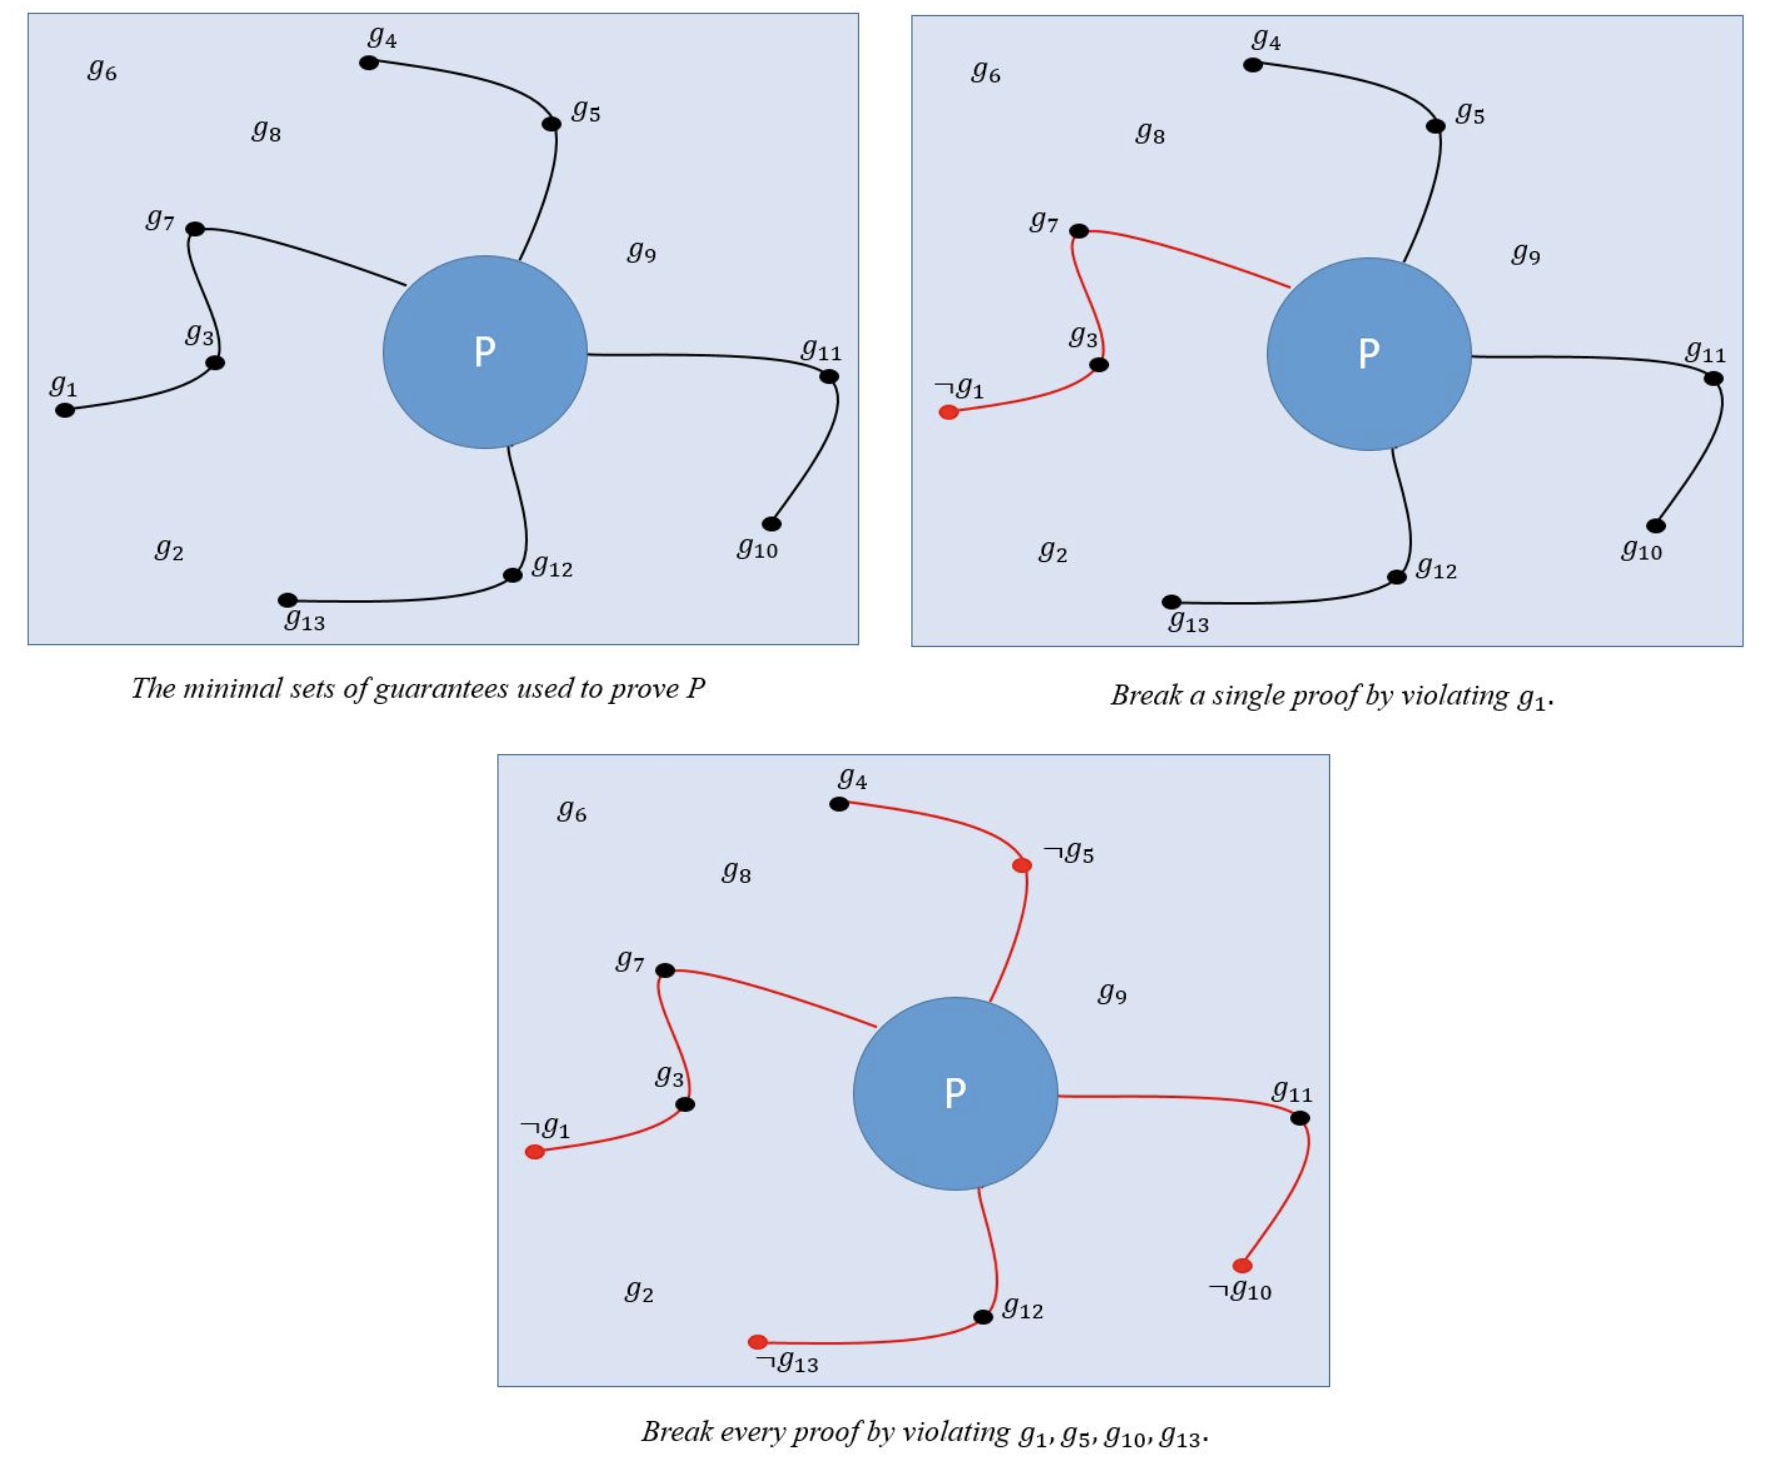
\includegraphics[width=0.9\textwidth]{images/mivcBreaking.png}
	\end{center}
	\caption{Using MIVCs to derive minimal cut sets}
	\label{fig:mivcBreaking}
\end{figure}

In Figure~\ref{fig:mivcBreaking}, we depict this graphically. In the first box (top left), the contracts of the single layer system are $g_1, \dots, g_{13}$. In this example, not all guarantees are needed to prove $P$; one may obtain proof of the property by having only $g_4$ and $g_5$ in the model. The \aivcalg algorithm provides all minimal validity cores which is shown as the lines running through the guarantees. 

One may attempt to ``break" a proof by violating a guarantee in a single MIVC as shown in the top right of the figure. This does break a proof, but given there are multiple MIVCs, it is not enough. The bottom figure shows our method: violate one guarantee from each MIVC set to ensure that the property can no longer be proven. The key idea is that the hitting sets of all MIVCs produces the minimal cut sets. 

Next we outline the formal background and toolsuite used in the implementation and then describe the algorithm that is implemented in the safety annex for AADL. 

\subsection{Background}
JKind is an open-source industrial infinite-state inductive model checker for safety properties~\cite{2017arXiv171201222G}. Models and properties in JKind are specified in Lustre~\cite{Halbwachs91:IEEE}, a synchronous dataflow language, using the theories of linear real and integer arithmetic. JKind uses SMT-solvers to prove and falsify multiple properties in parallel. The JKind model checker uses {\em
  $k$-induction} which unrolls the property $P$ over $k$ steps of the
transition system.

\begin{comment}
%For an arbitrary transition system $(I, T)$, computing reachability can be very expensive or even impossible. Thus, we need a more effective way of checking if a safety property $P$ is satisfied by the system. The key idea is to over-approximate reachability. If we can find an over-approximation that implies the property, then the property must hold. Otherwise, the approximation needs to be refined.

A good first approximation for reachability is the property itself.
That is, we can check if the following formulas hold:
\begin{gather}
  \forall s.~ I(s) \Rightarrow P(s)
  \label{eq:1-ind-base} \\
  \forall s, s'.~ P(s) \land T(s, s') \Rightarrow P(s')
  \label{eq:1-ind-step}
\end{gather}
If both formulas hold then $P$ is {\em inductive} and holds over the
system. If (\ref{eq:1-ind-base}) fails to hold, then $P$ is violated
by an initial state of the system. If (\ref{eq:1-ind-step}) fails to
hold, then $P$ is too much of an over-approximation and needs to be
refined.


The JKind model checker uses {\em
  $k$-induction} which unrolls the property $P$ over $k$ steps of the
transition system. For example, 1-induction consists of formulas (\ref{eq:1-ind-base}) and (\ref{eq:1-ind-step}) above, whereas 2-induction consists of the following formulas:
\begin{gather*}
\forall s.~ I(s) \Rightarrow P(s) \\
\forall s, s'.~ I(s) \land T(s, s') \Rightarrow P(s') \\
\forall s, s', s''.~ P(s) \land T(s, s') \land P(s') \land T(s',
  s'') \Rightarrow P(s'')
\end{gather*}
That is, there are two base step checks and one inductive step check.
In general, for an arbitrary $k$, $k$-induction consists of $k$
base step checks and one inductive step check as shown in
Figure~\ref{fig:k-induction} (the universal quantifiers on $s_i$ have
been elided for space). We say that a property is $k$-inductive if it
satisfies the $k$-induction constraints for the given value of $k$.
The hope is that the additional formulas in the antecedent of the
inductive step make it provable.

\begin{figure}
\begin{gather*}
I(s_0) \Rightarrow P(s_0) \\[-2pt]
%
\vdots \\[2pt]
%
I(s_0) \land T(s_0, s_1) \land \cdots \land T(s_{k-2}, s_{k-1})
\Rightarrow P(s_{k-1}) \\[2pt]
%
P(s_0) \land T(s_0, s_1) \land \cdots \land P(s_{k-1}) \land
T(s_{k-1}, s_k) \Rightarrow P(s_k)
\end{gather*}
\caption{$k$-induction formulas: $k$ base cases and one inductive
  step}
\label{fig:k-induction}
\end{figure}

In practice, inductive model checkers often use a combination of the
above techniques. Thus, a typical conclusion is of the form ``$P$ with
lemmas $L_1, \ldots, L_n$ is $k$-inductive''.
\end{comment}

Each step of induction is sent to an SMT (Satisfiabilty Modulo Theory)-solver to check for \emph{satisfiability}, i.e. there exists a total truth assignment to a given formula that evaluates to true. If there does not exist such an assignment, the formula is considered \emph{unsatisfiable}. %A \emph{constraint system} is a term used to describe the formula with all constraints to the variables. 
A $\mathit{k}$-induction model checker utilizes parallel SMT-solving engines at each induction step to glean information about the proof of a safety property. The transition formula is translated into clauses such that satisfiability is preserved~\cite{een2003temporal}. Expression of the base and induction steps of a temporal induction proof as SAT problems is straightforward and is shown below for step $k$:

\begin{gather*}
I(s_0) \land T(s_0, s_1) \land \cdots \land T(s_{k-1}, s_{k})
\land \neg P(s_{k})
\end{gather*}

When proving correctness it is shown that the formulas are \emph{unsatisfiable}, i.e., the property $P$ is provable. The idea behind finding an {\em inductive validity core} (IVC) for a given property $P$~\cite{GhassabaniGW16} is based on inductive proof methods used in SMT-based model checking, such as $\mathit{k}$-induction and IC3/PDR~\cite{een2011efficient, kahsai2012incremental, cook1971complexity}. Generally, an IVC computation technique aims to determine, for any subset $S \subseteq T$, whether $\mathit{P}$ is provable by $\mathit{S}$. A minimal subset that satisfies $\mathit{P}$ is seen as a minimal proof explanation and called a minimal inductive validity core. %Ghassabani et al. demonstrate that the minimization process is as hard as model checking~\cite{Ghassabani2017EfficientGO}, so finding a minimal inductive validity core may not be possible for some model checking problems. 

\begin{definition}
Inductive Validity Core (IVC)~\cite{GhassabaniGW16}: $S \subseteq T$ for $(I, T) \vdash P$ is an Inductive Validity Core, denoted by $\mathit{IVC(P,S)}$, iff $\mathit{(I,S)} \vdash P$.
\end{definition}

\begin{definition}
Minimal Inductive Validity Core (MIVC)~\cite{Ghassabani2017EfficientGO}: $S \subseteq T$ is a minimal Inductive Validity Core, denoted by $\mathit{MIVC(P,S)}$, iff $\mathit{IVC(P,S)} \land \forall T_i \in S$. $(I, S \setminus \{T_i\}) \not \vdash P$.
\end{definition}

The {\em constraint system} consists of the constrained formulas of the transition system and the negation of the property. The \aivcalg algorithm collects all {\em minimal unsatisfiable subsets} (MUSs) of a constraint system generated from a transition system at each induction step~\cite{Ghassabani2017EfficientGO,bendik2018online}. 

\begin{definition}
A Minimal Unsatisfiable Subset (MUS)~\cite{reiter1987theory} $M$ of a constraint system $C$ is a set $M \subseteq C$ such that $M$ is unsatisfiable and $\forall c \in M$ : $M \setminus \{c\}$ is satisfiable.
\end{definition}
The MUSs are the minimal explanation of the infeasibility of this constraint system; equivalently, these are the minimal sets of model elements necessary for proof of the safety property.

Returning to our running example, this can be illustrated by the following. Given the constraint system $C = \{G_p, G_t, G_r, \neg P\}$, a minimal explanation of the infeasability of this system is the set $\{G_p, G_t, G_r,\}$. If all three guarantees hold, then $P$ (the disjunction of these guarantees) is provable. 

In the case of an UNSAT system, we may ask: what will correct this unsatisfiability? A related set answers this question: 
\begin{definition}
A Minimal Correction Set (MCS)~\cite{reiter1987theory} $M$ of a constraint system $C$ is a subset $M\subseteq C$ such that $C \setminus M$ is satisfiable and $\forall M' \subset M$ : $C \setminus M'$ is unsatisfiable.
\end{definition}
A MCS can be seen to ``correct'' the infeasability of the constraint system by the removal from $C$ the constraints found in an MCS. Returning to the PWR example, the MCSs of the constraint system $C$ are $\mathit{MCS}_1 = \{G_t\}$, $\mathit{MCS}_2 = \{G_p\}$, $\mathit{MCS}_3 = \{G_r\}$. If any single guarantee is violated, a shut down from that subsystem may not get sent when it should and the safety property $P$ will be violated. This corresponds exactly to the definition of a minimal cut set.

For the following definitions, we remind readers of the extended transition system defined in Equation 2 of Section~\ref{sec:formalization} and that the elements of $T$ are the set $\mathit{GF} \cup \mathit{AF}$ for potentially faulty guarantees $\mathit{GF}$ and activation literals $\mathit{AF}$. We use the notation $\mathit{af} \rightarrow \{\mathit{true}, \mathit{false}\}$ to indicate a constraint on the literal $\mathit{af}$. 

\begin{definition}
A cut set $S$ of a top level event $\neg P$ is a set $S \subseteq \mathit{AF}$ such that $\forall \mathit{af} \in S$, $\mathit{af} \rightarrow \{\mathit{true}\}$ and $S \cup \{\neg P\}$ is satisfiable.
\end{definition}

Intuitively, a cut set is a true valuation for some subset of fault activation literals within a constraint system such that the constraint system is satisfiable given those true valuations.

\begin{definition}
A cut set $S$ is minimal if and only if $\forall \mathit{af} \in S$, $S \setminus \{\mathit{af}\} \cup \{\neg P\}$ is unsatisfiable.
\end{definition}

Our approach in computing minimal cut sets through the use of inductive validity cores is to supply activation literals constrained to be false to the algorithm. The resulting $\mathit{MCS}s$ consist of elements $\neg \mathit{af}_i$. The removal of this constraint from the constraint system results in non-deterministically true activation literals. By the definition of an $\mathit{MCS}$, we know that $C \setminus \mathit{MCS}$ is satisifiable. This removal of constraints from $C$ removes the {\em false} constraint from each element in the $\mathit{MCS}$. Liffiton et. al showed that any subset of a satisfiable set is also satisfiable~\cite{liffiton2016fast}, so we know that for set $S$ consisting of elements of $\mathit{MCS}$ with constraints removed, $S \cup \{\neg P\}$ is also satisfiable. This is the definition of a cut set. Minimality comes directly from the definition of a minimal correction set. 

A duality exists between the MUSs of a constraint system and the MCSs as established by Reiter \cite{reiter1987theory}. This duality is defined in terms of \textit{Minimal Hitting Sets} (\textit{MHS}). 
\begin{definition}
A hitting set of a collection of sets $A$ is a set $H$ such that every set in $A$ is ``hit'' by $H$; $H$ contains at least one element from every set in $A$. 
\end{definition}
Every MUS of a constraint system is a minimal hitting set of the system's MCSs, and likewise every MCS is a minimal hitting set of the system's MUSs. This is noted in previous work~\cite{liffiton2016fast, de1987diagnosing} and the proof of such is given by Reiter (Theorem 4.4 and Corollary 4.5)~\cite{reiter1987theory}. For the PWR top level constraint system, it can be seen that each of the MCSs intersected with the MUS is nonempty. This gives the minimal set of guarantees for which, if violated, will cause $P$ to be violated. 

As described in Section~\ref{sec:formalization}, we extend the transition system with fault activation literals. These literals are constrained to {\em false} and the \aivcalg algorithm is invoked. The constraint system for the PWR example is $C = \{\neg\mathit{af}_p, \neg\mathit{af}_t, \neg\mathit{af}_r, \neg P\}$ for activation literal $\mathit{af}_p$ associated with $G_p$, etc. The hitting sets generated from the MIVC are: $\{\neg\mathit{af}_p\}$, $\{\neg\mathit{af}_t\}$, and $\{\neg\mathit{af}_r\}$ and are the minimal correction sets of the constraint system. 

%\textbf{Background Information on Toolsuite}
\danielle{My suggestion is to place this at the front of the implementation section. It just seems like it is taking longer to get to the interesting part of the paper by having it here.}

The algorithms in this paper are implemented in the Safety Annex for the Architecture Analysis and Design Language (AADL) and require the Assume-Guarantee Reasoning Environment (AGREE)~\cite{NFM2012:CoGaMiWhLaLu} to annotate the AADL model in order to perform verification using the back-end model checker \jkind~\cite{2017arXiv171201222G}. 

\textbf{Architecture Analysis and Design Language}
We are using the Architectural Analysis and Design Language (AADL) to construct system architecture models of performance-critical, embedded, real-time systems~\cite{AADL_Standard,FeilerModelBasedEngineering2012}. %An AADL model describes a system in terms of a hierarchy of components and their interconnections, where each component can either represent a logical entity (e.g., application software functions, data) or a physical entity (e.g., buses, processors). 
Language annexes to AADL provide a richer set of modeling elements for various system design and analysis needs, and the language definition is sufficiently rigorous to support formal analysis tools that allow for early phase error/fault detection. 

\textbf{Compositional Analysis} 
One way to structure compositional verification is hierarchically: layers of the system architecture are analyzed independently and their composition demonstrates a system property of interest. Compositional verification partitions the formal analysis of a system architecture into verification tasks that correspond into the decomposition of the architecture~\cite{clarke1989compositional}.  A proof consists of demonstrating that the system property is provable given the contracts of its direct subcomponents and the system assumptions~\cite{cofer2012compositional,clarke1989compositional}. When compared to monolithic analysis (i.e., analysis of the flattened model composed of all components), the compositional approach allows the analysis to scale to much larger systems~\cite{NFM2012:CoGaMiWhLaLu,heckel1998compositional,cofer2012compositional}.

\textbf{Assume Guarantee Reasoning Environment}
The Assume Guarantee Reasoning Environment (AGREE) is a tool for formal analysis of behaviors in AADL models and supports compositional verification~\cite{NFM2012:CoGaMiWhLaLu}.  It is implemented as an AADL annex and is used to annotate AADL components with formal behavioral contracts. Each component's contracts includes assumptions and guarantees about the component's inputs and outputs respectively. AGREE translates an AADL model and the behavioral contracts into Lustre~\cite{Halbwachs91:IEEE} and then queries the \jkind model checker to conduct the back-end analysis~\cite{2017arXiv171201222G}. 

\textbf{JKind}
JKind is an open-source industrial infinite-state inductive model checker for safety properties~\cite{2017arXiv171201222G}. Models and properties in JKind are specified in Lustre~\cite{Halbwachs91:IEEE}, a synchronous dataflow language, using the theories of linear real and integer arithmetic. JKind uses SMT-solvers to prove and falsify multiple properties in parallel.

\textbf{Safety Annex for AADL}
The Safety Annex for AADL provides the ability to reason about faults and faulty component behaviors in AADL models~\cite{Stewart17:IMBSA,stewart2020safety}. In the Safety Annex approach, AGREE is used to define the nominal behavior of system components, faults are introduced into the nominal model, and JKind is used to analyze the behavior of the system in the presence of faults. Faults describe deviations from the nominal behavior and are attached to the outputs of components in the system.%The Safety Annex supports behavioral specification of faults and their implicit propagation through behavioral relationships in the model as well as explicit propagation through dependencies. 




\section{Fault Modeling with the Safety Annex}
\label{sec:fault_modeling}

To demonstrate the fault modeling capabilities of the Safety Annex we will use the Wheel Brake System (WBS) described in AIR6110~\cite{AIR6110}.  This system is a well-known example that has been used as a case study for safety analysis, formal verification, and contract based design~\cite{DBLP:conf/cav/BozzanoCPJKPRT15, 10.1007/978-3-319-11936-6-7, CAV2015:BoCiGrMa, Joshi05:SafeComp}. %The preliminary work for the safety annex was based on a simple model of the WBS~\cite{Stewart17:IMBSA}. To demonstrate a more complex fault modeling process, we constructed a functionally and structurally equivalent AADL version of one of the more complex WBS NuSMV/xSAP model (arch4wbs)~\cite{DBLP:conf/cav/BozzanoCPJKPRT15}.    

\begin{figure}[h!]
	\centering
	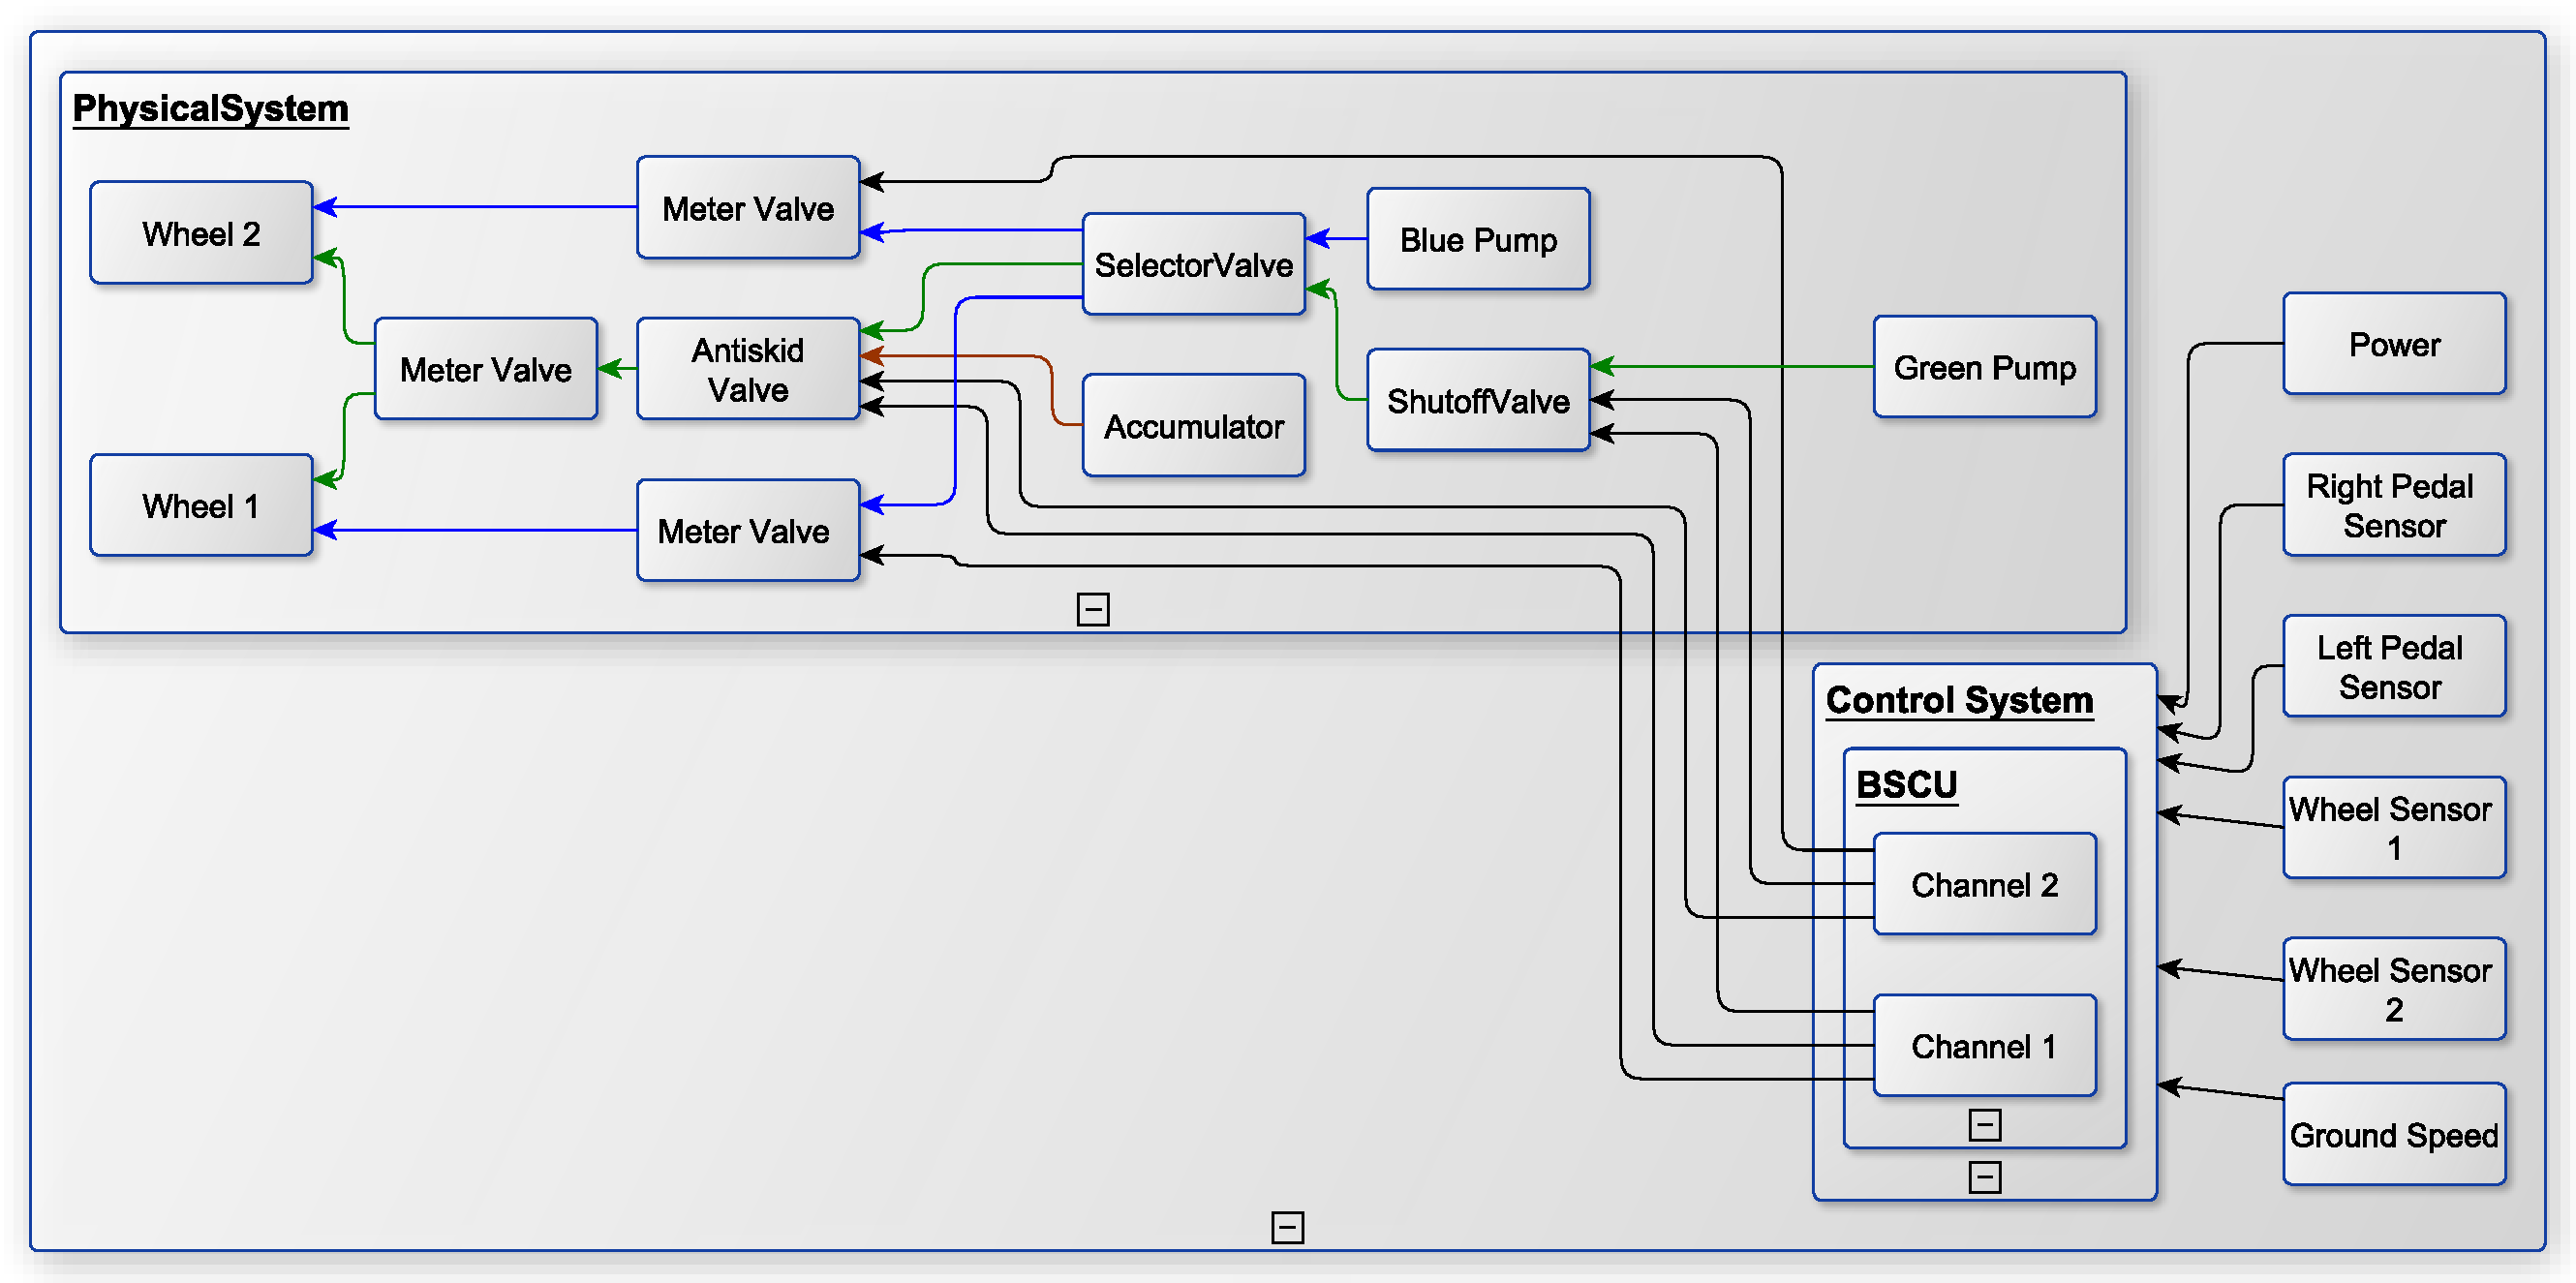
\includegraphics[trim=0 9 0 5,clip,width=\textwidth]{images/wbs_arch4_diagram.pdf}
	\caption{Wheel Brake System}
	\label{fig:wbs}
\end{figure} 

The WBS is composed of two main parts: the Line Replaceable Unit control system and the electro-mechanical physical system.
The control system electronically controls the physical system and contains a redundant
channel of the Braking System Control Unit (BSCU) in case a detectable fault occurs in the active channel.
 It also commands antiskid braking.% in case of skidding on the ground. 
The physical system consists of the hydraulic circuits running from hydraulic pumps to wheel brakes as well as valves that control the hydraulic fluid flow. This system provides braking force to each of the eight wheels of the aircraft. The wheels are all mechanically braked in pairs (one pair per landing gear). For simplicity, Figure~\ref{fig:wbs} displays only two of the eight wheels. 

There are three operating modes in the WBS model:

\begin{itemize}
	\renewcommand{\labelitemi}{\textbullet}
	\item In \textit{normal} mode, the system is composed of a \textit{green} hydraulic pump and one meter valve per each of the eight wheels. Each of the meter valves are controlled through electronic commands coming from the active channel of the BSCU. These signals provide braking and antiskid commands for each wheel. The braking command is determined through a sensor on the pedal and the antiskid command is determined by the \textit{Wheel Sensors}. 
	\item In \textit{alternate} mode, the system is composed of a \textit{blue} hydraulic pump, four meter valves, and four antiskid shutoff valves, one for each landing gear. The meter valves are mechanically commanded through the pilot pedal corresponding to each landing gear. If the system detects lack of pressure in the green circuit, the BSCU channel commands the selector valve to switch to the blue circuit. 
	\item In \textit{emergency} mode, the system mode is entered if the \textit{blue} hydraulic pump fails. The accumulator pump has a reserve of pressurized hydraulic fluid and will supply this to the blue circuit in emergency mode. 
\end{itemize}

The WBS architecture model in AADL contains 30 different kinds of components, 169 component instances, and a model depth of 5 hierarchical levels. 


%If the BSCU channel becomes invalid, the shutoff valve closes and we move into alternate mode. Once this system switches into alternate mode, it does not return to normal operation mode.

%There are three operating modes in the WBS model. In \textit{normal} mode, the system uses the \textit{green} hydraulic circuit. The normal system is composed of the green hydraulic pump and one meter valve per each of the eight wheels. Each of the meter valves are controlled through electronic commands coming from the active channel of the BSCU. These signals provide braking and antiskid commands for each wheel. The braking command is determined through a sensor on the pilot pedal position and is labeled as \textit{Left/Right Pedal Sensor} in Figure~\ref{fig:wbs} and the antiskid command is determined by the \textit{Wheel Sensors}. 

%In \textit{alternate} mode, the system uses the \textit{blue} hydraulic circuit. The alternate system is composed of the blue hydraulic pump, four meter valves, and four antiskid shutoff valves: one for each landing gear. The meter valves are mechanically commanded through the pilot pedal corresponding to each landing gear. If the system detects lack of pressure in the green circuit, the BSCU channel commands the selector valve to switch to the blue circuit. 
%If the BSCU channel becomes invalid, the shutoff valve closes and we move into alternate mode. Once this system switches into alternate mode, it does not return to normal operation mode.

%The last mode of operation of the WBS is the \textit{emergency} mode. This mode is entered if the blue hydraulic pump fails. The accumulator pump has a reserve of pressurized hydraulic fluid and will supply this to the blue circuit in emergency mode.

%The model contains 30 different kinds of components, 169 component instances, a model depth of 5 hierarchical levels.  The model includes one top-level assumption and  11 top-level system properties, with 113 guarantees allocated to subsystems.  There are a total of 33 different fault types and 141 fault instances within the model.  The large number of fault instances is due to the redundancy in the system design and its replication to control 8 wheels.

The behavioral model is encoded using the AGREE annex and the behavior is based on descriptions found in AIR6110. The top level system properties are given by the requirements and safety objectives in AIR6110. All of the subcomponent contracts support these system safety objectives through the use of assumptions on component input and guarantees on the output. The WBS behavioral model in AGREE annex includes one top-level assumption and  11 top-level system properties, with 113 guarantees allocated to subsystems.  

An example system safety property is to ensure that there is no inadvertent braking of any of the wheels. This is based on a failure condition described in AIR6110 is \textit{Inadvertent wheel braking on one wheel during takeoff shall be less than 1E-9 per takeoff}. 
Inadvertent braking means that braking force is applied at the wheel but the pilot has not pressed the brake pedal.  In addition, the inadvertent braking requires that power and hydraulic pressure are both present, the plane is not stopped, and the wheel is rolling (not skidding). 
%in Figure~\ref{fig:inadvertent_braking}. 
The property is stated in AGREE such that inadvertent braking does \textit{not} occur, as shown below. 

\begin{figure}[h!]
	\vspace{-0.2in}
	\begin{center}
		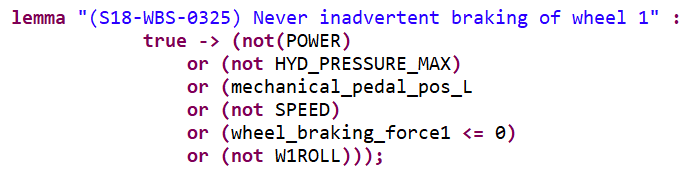
\includegraphics[width=.7\textwidth]{images/inadvertent_braking.png}
	\end{center}
	\vspace{-0.3in}
	%\caption{AGREE Contract for Top Level Property}
	\label{fig:inadvertent_braking}
	%\vspace{-0.2in}
\end{figure}


\subsection{Component Fault Modeling}

The usage of the terms error, failure, and fault are defined in ARP4754A and are described here for ease of understanding~\cite{SAE:ARP4754A}. An \textit{error} is a mistake made in implementation, design, or requirements. A \textit{fault} is the manifestation of an error and a \textit{failure} is an event that occurs when the delivered service of a system deviates from correct behavior. If a fault is activated under the right circumstances, that fault can lead to a failure. The terminology used in EMV2 differs slightly for an error: an error is a corrupted state caused by a fault. The error propagates through a system and can  manifest as a failure. In this paper, we use the ARP4754A terminology with the added definition of \textit{error propagation} as used in EMV2. An error is a mistake made in design or code and an error propagation is the corrupted state caused by an active fault. 

The Safety Annex is used to add potential faulty behaviors to a component model.  When the fault is activated by its specified triggering conditions, it modifies the output of the component. This faulty behavior may violate the contracts of other components in the system, including assumptions of downstream components. The impact of a fault is computed by the AGREE model checker when the safety analysis is run on the fault model. Examples of such faults include valves being stuck open or closed, output of a software component being nondeterministic, or power being cut off. 
%Faulty components can be mechanical or digital, but in this section we focus on a digital component in the WBS -- a brake pedal position sensor component. 

One of the components important to the inadvertent braking property is the brake pedal. When the mechanical pedal is pressed, a sensor reads this information and passes an electronic signal to the BSCU which then commands hydraulic pressure to the wheels. 

%Figure~\ref{fig:sensor} 
Below shows the AADL pedal sensor component with a contract for its nominal behavior. The sensor has only one input, the mechanical pedal position, and one output, the electrical pedal position. %The 
A property that governs the behavior of the component is that the mechanical position should always equal the electronic position. 

\begin{figure}[h!]
	\hspace*{-2cm}
	\vspace{-0.55in} 
	\begin{center}
		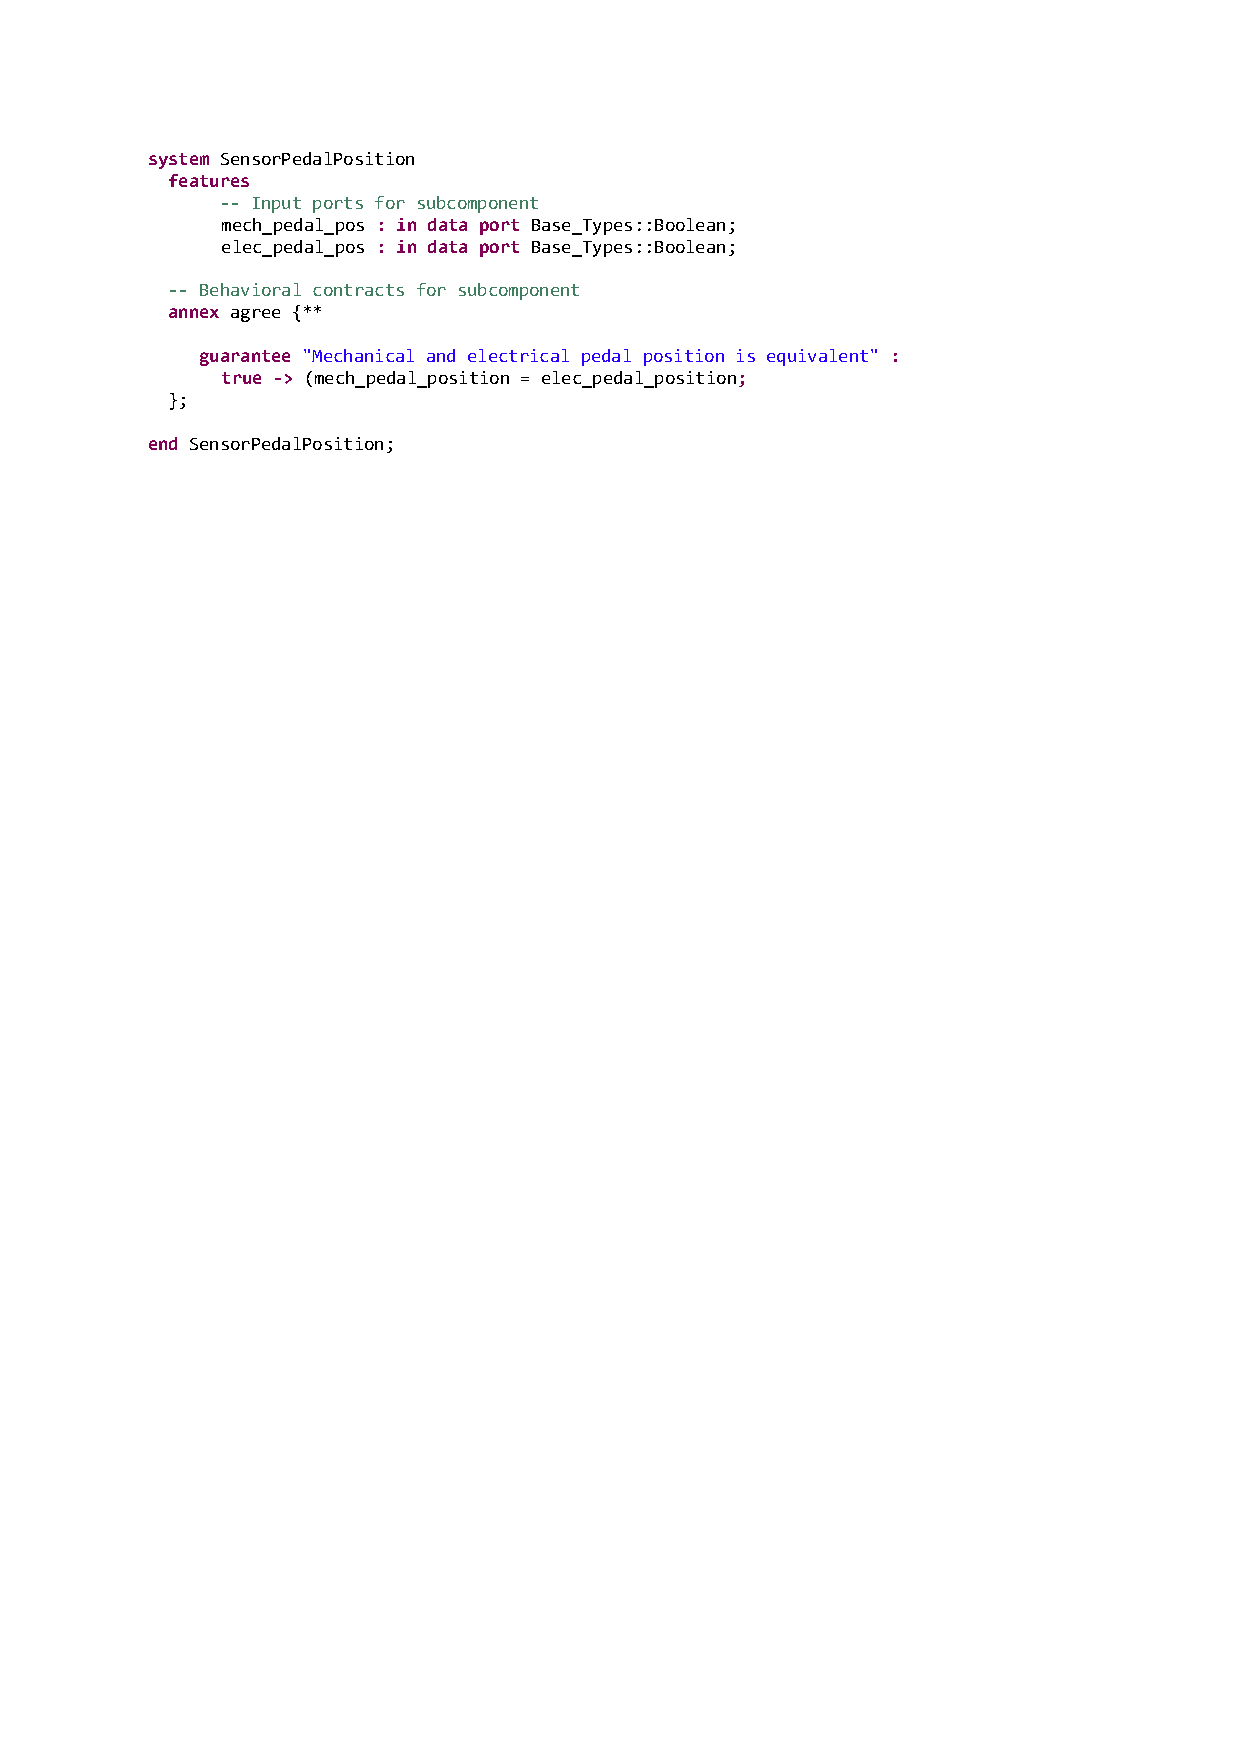
\includegraphics[trim=0 640 -10 70,clip,width=1.5\dimexpr\textwidth-2cm\relax]{images/system_sensor.pdf}
		\vspace{-0.3in}
	%	\caption{An AADL System Type: The Pedal Sensor}
		\label{fig:sensor}
	\end{center}
	\vspace{-0.2in}
\end{figure}

One possible failure for this sensor is inversion of its output value. This fault can be triggered with probability $5.0\times 10^{-6}$ as described in AIR6110 (in reality, the component failure probability is 
collected from hardware specification sheets).  %Figure~\ref{fig:sensorFault} 
The Safety Annex definition for this fault is shown below. Fault behaviors may be defined by the user or by using a library of fault nodes, in this case, \textit{inverted\_fail}.  When the fault is triggered, the nominal output of the component (\textit{elec\_pedal\_position}) is replaced with its failure value (\textit{val\_out}). 

\begin{figure}[h!]
	\hspace*{-2cm}
	\vspace{-0.5in} 
	\begin{center}
		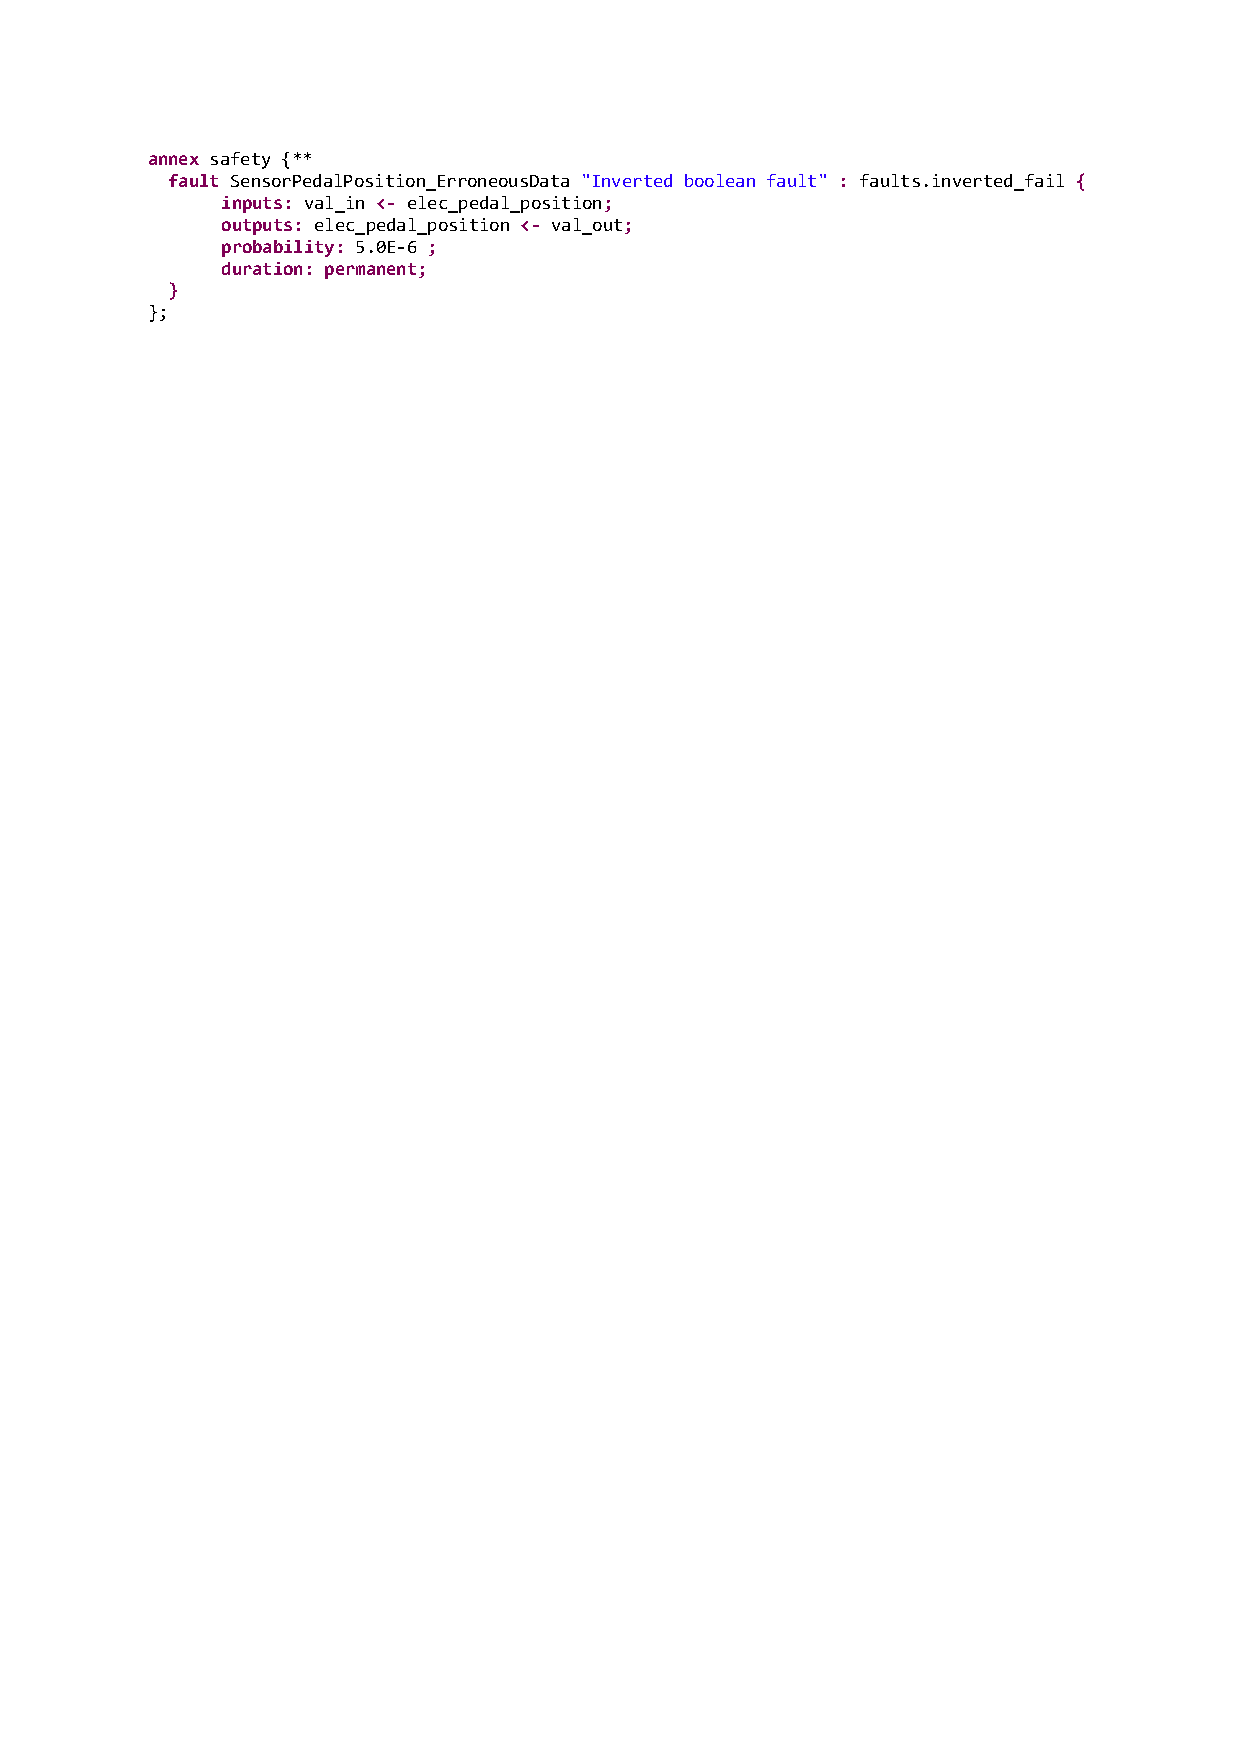
\includegraphics[trim=0 680 -10 70,clip,width=1.5\dimexpr\textwidth-2cm\relax]{images/safetyannex_sensorfault.pdf}
		%\vspace{-0.3in}
		%\caption{The Safety Annex for the Pedal Sensor}
		\label{fig:sensorFault}
	\end{center}
	\vspace{-0.5in}
\end{figure}

The WBS fault model in Safety Annex contains a total of 33 different fault types and 141 fault instances. The large number of fault instances is due to the redundancy in the system design and its replication to control 8 wheels.

\subsection{Implicit %Failure
	Error Propagation}
In the Safety Annex approach, faults are captured as faulty behaviors that augment the system behavioral model in AGREE contracts. No explicit %fault
error propagation is necessary since the faulty behavior itself propagates through the system just as in the nominal system model. The effects of any triggered fault are manifested through analysis of the AGREE contracts. 

On the contrary, in the AADL Error Model Annex, Version 2 (EMV2)~\cite{EMV2} approach, all errors must be explicitly propagated through each component (by applying fault types on each of the output ports) in order for a component to have an impact on the rest of the system. To illustrate the key differences between implicit %failure
error propagation provided in Safety Annex and the explicit %failure 
error propagation provided in EMV2, we use a simplified behavioral flow from the WBS example using code fragments from EMV2, AGREE, and the Safety Annex. 

\begin{figure}[t]
	\vspace{-0.19in}
	\centering
	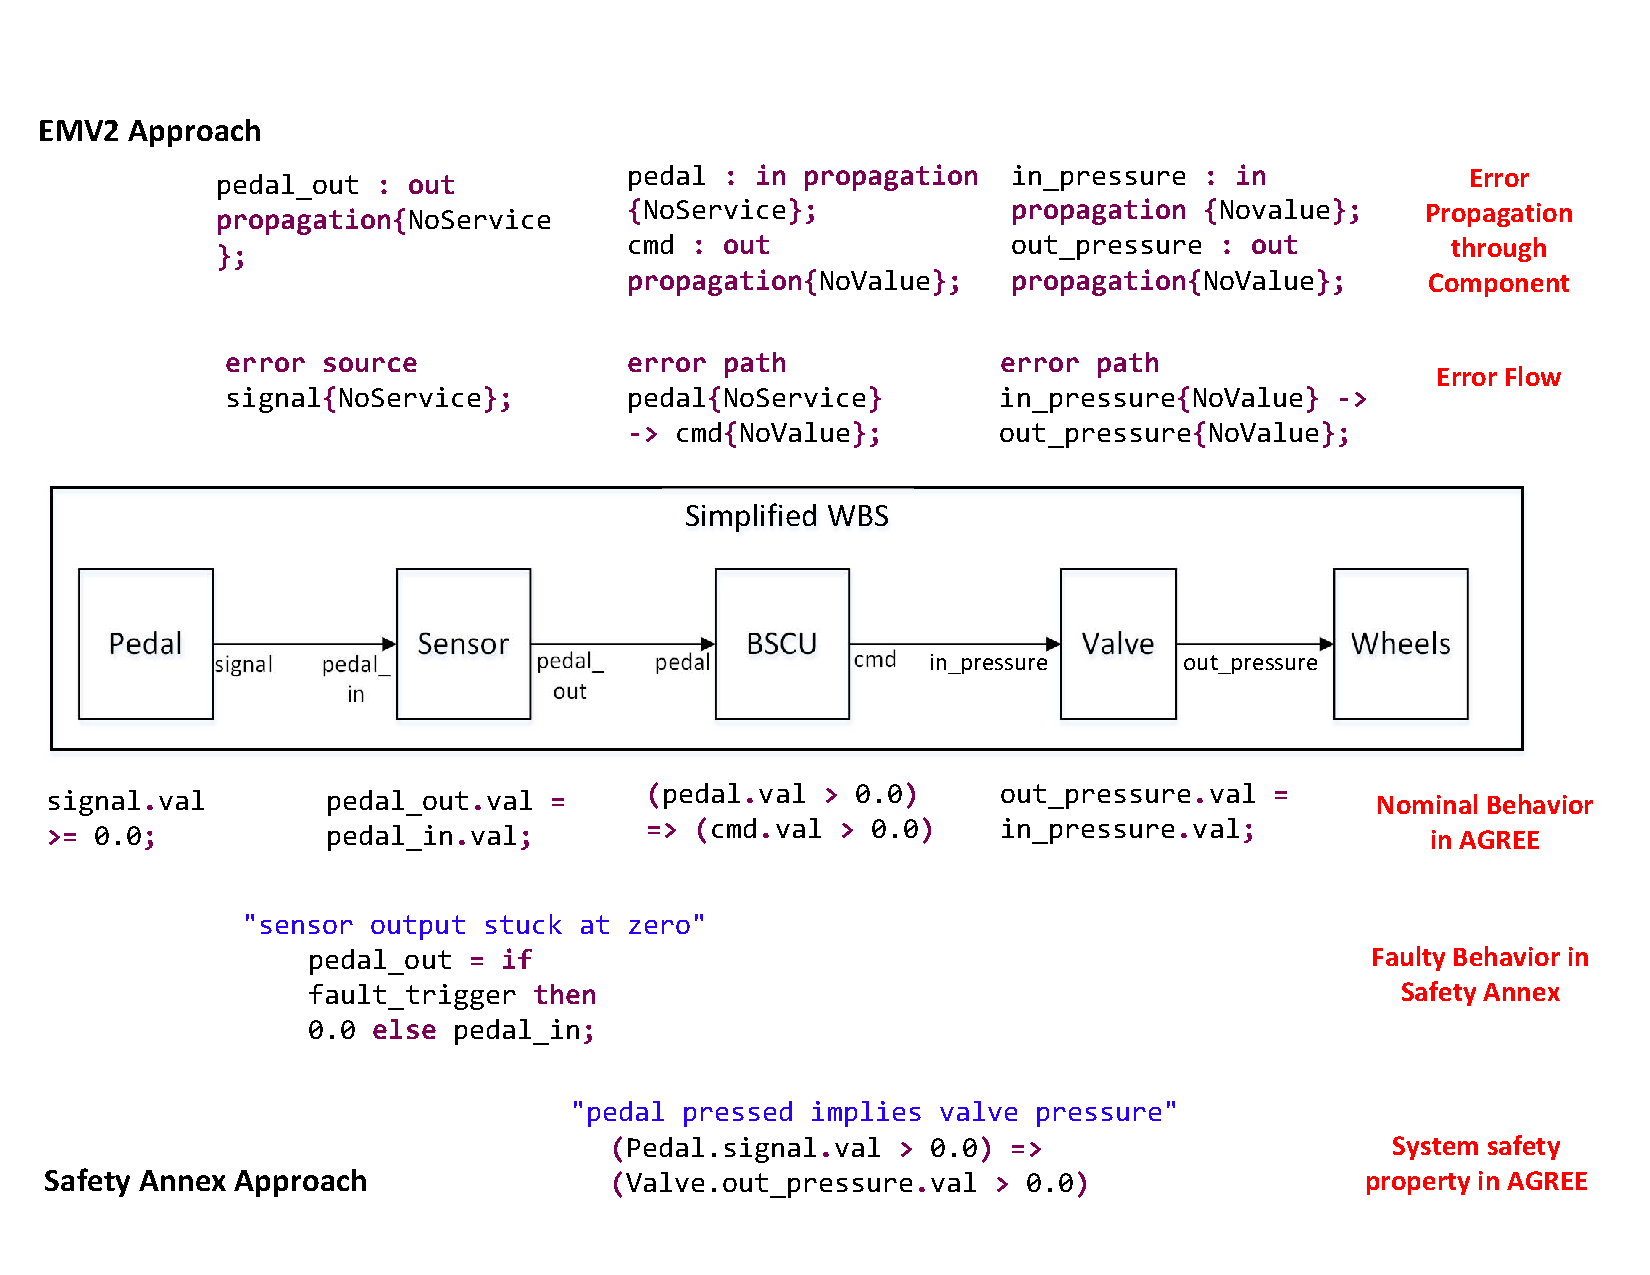
\includegraphics[trim=0 9 0 5,clip,width=\textwidth]{images/Comparison_with_EMV2.pdf}
	\vspace{-0.3in}
	\caption{Differences between Safety Annex and EMV2}
	\label{fig:comparison_with_EMV2}
	\vspace{-0.2in}
\end{figure} 

In this simplified WBS system, the physical signal from the Pedal component is detected by the Sensor and the pedal position value is passed to the Braking System Control Unit (BSCU) components.  The BSCU generates a pressure command to the Valve component which applies hydraulic brake pressure to the Wheels. 

In the EMV2 approach (top half of Figure~\ref{fig:comparison_with_EMV2}), the ``NoService'' fault is explicitly propagated through all of the components. These fault types are essentially tokens that do not capture any analyzable behavior. At the system level, analysis tools supporting the EMV2 annex can aggregate the propagation information from different components to compose an overall fault flow diagram or fault tree. 

When a fault is triggered in the Safety Annex (bottom half of Figure~\ref{fig:comparison_with_EMV2}), the output behavior of the Sensor component is modified. In this case the result is a ``stuck at zero'' error. The behavior of the BSCU receives a zero input and proceeds as if the pedal has not been pressed. This will cause the top level system contract to fail: {\em pedal pressed implies brake pressure output is positive}.

\begin{comment}
%\subsection{Comparison to the AADL Error Annex}

The AADL language has previously been extended to provide some fault modeling and analysis capabilities using its Error Model Annex, Version 2 (EMV2)~\cite{EMV2}.  EMV2 focuses on injection and propagation of discrete faults for generation of fault trees, rather than on analysis of system behavior in the presence of faults. 
To illustrate some of the key differences between our approach and the EMV2 approach, Figure~\ref{fig:comparison_with_EMV2} shows a simplified  behavioral flow with code fragments from EMV2, AGREE, and the Safety Annex. 

\begin{figure}[t]
	\vspace{-0.45in}
	\centering
	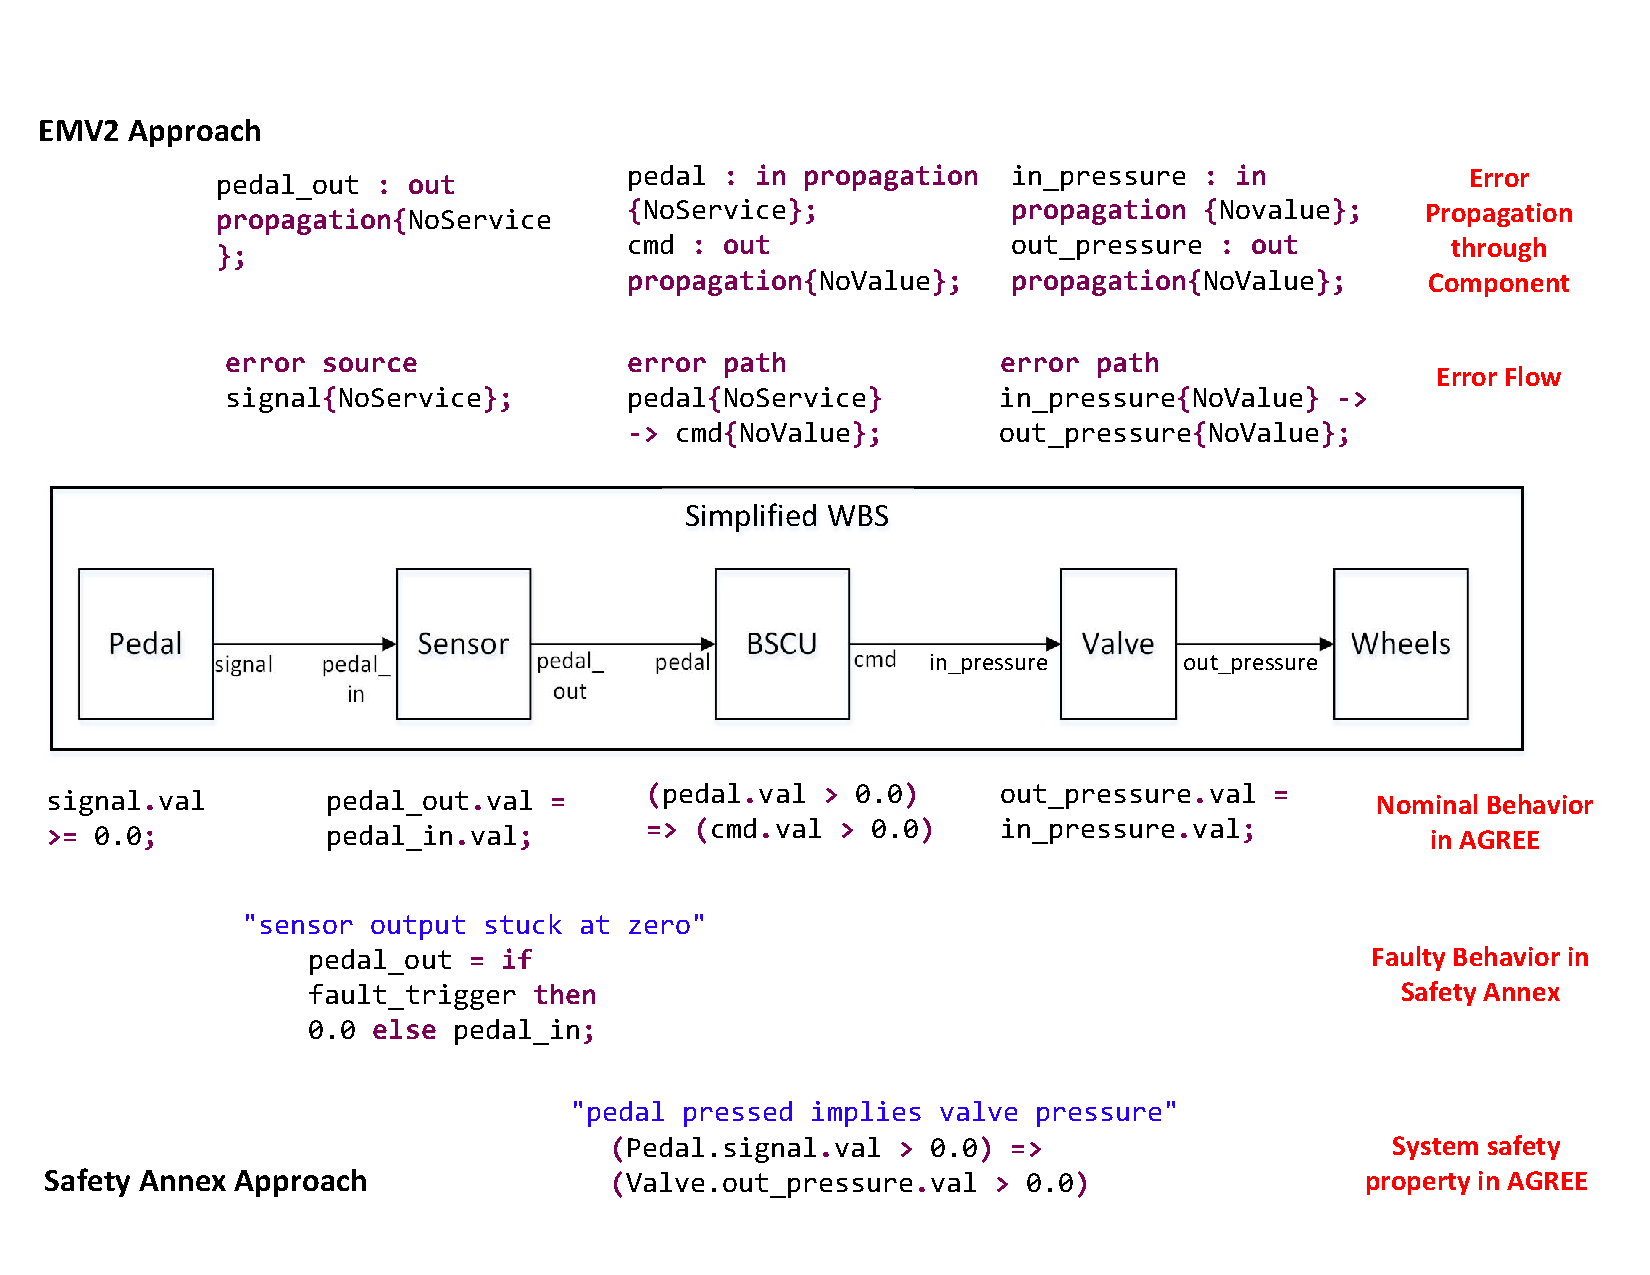
\includegraphics[trim=0 9 0 5,clip,width=\textwidth]{images/Comparison_with_EMV2.pdf}
	%\vspace{0.4in}
	\caption{Differences between Safety Annex and EMV2}
	\label{fig:comparison_with_EMV2}
\end{figure} 

In this simplified WBS system, the physical signal from the Pedal component is detected by the Sensor, and the pedal position value is passed to the Braking System Control Unit (BSCU) components.  The BSCU generates a pressure command to the Valve component which applies hydraulic brake pressure to the Wheels. 

In the EMV2 approach (top half of Figure~\ref{fig:comparison_with_EMV2}), all errors must be explicitly propagated through each component (by applying fault types on each of the output ports) in order for a component to have an impact on the rest of the system. In the example, the ``NoService'' fault is explicitly allowed by the EMV2 declarations to propagate through all of the components.  These fault types are essentially tokens that do not capture any analyzable behavior.  At the system level, analysis tools supporting the EMV2 annex can aggregate the fault flow and propagation information from different components to compose an overall fault flow diagram or fault tree.

In the Safety Annex approach (bottom half of Figure~\ref{fig:comparison_with_EMV2}), faults augment the system behavioral model through the AGREE contracts.  When a fault is triggered, the output behavior of the Sensor component is modified, in this case resulting a ``stuck at zero'' error. The behavior of the BSCU receives a zero input and proceeds as if the pedal has not been pressed. This will cause the top level system contract to fail: {\em pedal pressed implies brake pressure output is positive}. No explicit propagation is necessary since the faulty behavior propagates through the system just as in the nominal system model. The system and component failures are manifested through analysis of the AGREE contracts. 
\end{comment}

\subsection{Explicit %Failure 
	Error Propagation} 
%Faults
Failures in hardware (HW) components can trigger behavioral faults in the system components that depend on them. For example, a CPU %fault
Failure may trigger faulty behavior in the threads bound to that CPU. In addition, a %fault
failure in one HW component may trigger %faults
failure in other HW components located nearby, such as overheating, fire, or explosion
in the containment location. 
The Safety Annex provides the capability to explicitly model the impact of hardware %faults
failures on other faults, behavioral or non behavioral. The explicit propagation to non behavioral faults is similar to that provided in EMV2.

To better model %HW dependent faults 
faults at the system level dependent on HW failures, a fault model element is introduced called a \textit{hardware fault}. Users are not required to specify behavioral effects for the HW faults, nor are data ports necessary on which to apply the fault definition. An example of a model component fault declaration is shown below:
\begin{figure}[h!]
	\vspace{-0.2in}
	\begin{center}
	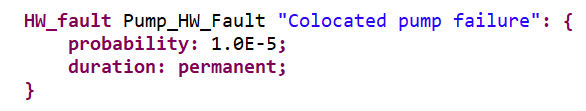
\includegraphics[width=.6\textwidth]{images/hw_fault2.png}
	\end{center}
	\vspace{-0.3in}
	%\caption{Hardware Fault Definition}
	\label{fig:hwFault}
	%\vspace{-0.2in}
	\vspace{-0.1in}
\end{figure}

Users specify dependencies between the HW component faults and faults that are defined in other components, either HW or SW. The hardware fault then acts as a trigger for dependent faults. This allows a simple propagation from the faulty HW component to the SW components that rely on it, affecting the behavior on the outputs of the affected SW components.

%As an example, we will look yet again at the WBS. 
In the WBS example, assume that both the green and blue hydraulic pumps are located in the same compartment in the aircraft and an explosion in this compartment rendered both pumps inoperable.
%An accident took place and the green (normal) hydraulic pump took the force of an explosion. When the green hydraulic pump exploded, the pump shrapnel flew into the blue pump and it became from then on unoperable. 
The HW fault definition can be modeled first in the green hydraulic pump component as shown in Figure~\ref{fig:hwFault}. The activation of this fault triggers the activation of related faults as seen in the \textit{propagate\_to} statement shown below. % in Figure~\ref{fig:hwFaultProp}. 
Notice that these pumps need not be connected through a data port in order to specify this propagation. %Furthermore, the probability of the HW fault activation can be specified. 

\begin{figure}[h!]
	\vspace{-0.2in}
	\begin{center}
		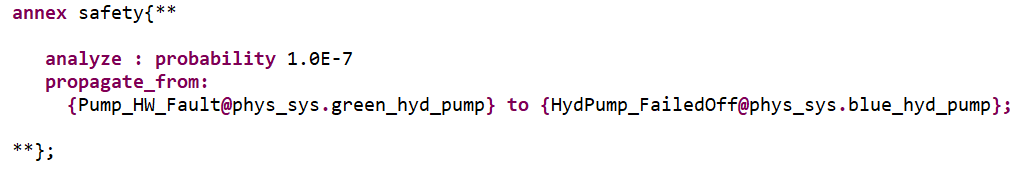
\includegraphics[width=1.0\textwidth]{images/hw_prop_stmt.png}
	\end{center}
	\vspace{-0.3in}
	%\caption{Hardware Fault Propagation Statement}
	\label{fig:hwFaultProp}
	%\vspace{-0.2in}
	\vspace{-0.1in}
\end{figure}

The fault dependencies are specified in the system implementation where the system configuration that causes the dependencies becomes clear (e.g., binding between SW and HW components, co-location of HW components). 
%This is because fault propagations are typically tied to the way components are connected or bound together; this information may not be available when faults are being specified for individual components. Having fault propagations specified outside of a component’s fault statements also makes it easier to reuse the component in different systems. 


\begin{comment}
\subsection{Fault Hypothesis}

An annotation in the AADL model determines the fault hypothesis. This may specify either a maximum number of faults that can be active at any point in execution (see Figure~\ref{fig:hwFaultProp}) or that only faults whose probability of simultaneous occurrence is above some probability threshold should be considered. Tying back to traditional safety analysis, the former is analogous to restricting the cutsets to a specified maximum number of terms, and the latter is analogous to restricting the cutsets to only those whose probability is above some set value.

In the former case, we assert that the sum of the true {\em fault\_\_trigger} variables is below some integer threshold.  In the latter, we determine all combinations of faults whose probabilities are above the specified probability threshold, and describe this as a proposition over {\em fault\_\_trigger} variables. 
%
With the introduction of dependent faults, active faults are divided into two categories: independently active (activated by its own triggering event) and dependently active (activated when the faults they depend on become active). The top level fault hypothesis applies to independently active faults. Faulty behaviors augment nominal behaviors whenever their corresponding faults are active (either independently active or dependently active).
\end{comment}










\section{Architecture and Implementation}
\label{sec:implementation}

The Safety Annex is written in Java as a plug-in for the OSATE AADL toolset, which is built on Eclipse.  It is not designed as a stand-alone extension of the language, but works with behavioral contracts specified in AGREE AADL annex~\cite{NFM2012:CoGaMiWhLaLu}. 
The architecture of the Safety Annex is shown in Figure~\ref{fig:plugin-arch}.

 %AGREE allows {\em assume-guarantee} behavioral contracts to be added to AADL components.  The language used for contract specification is based on the Lustre dataflow language~\cite{Halbwachs91:IEEE}. %AGREE improves scalability of formal verification to large systems by decomposing the analysis of a complex system architecture into a collection of smaller verification tasks that correspond to the structure of the architecture.

%\begin{comment}

\begin{figure}
	\begin{center}
		%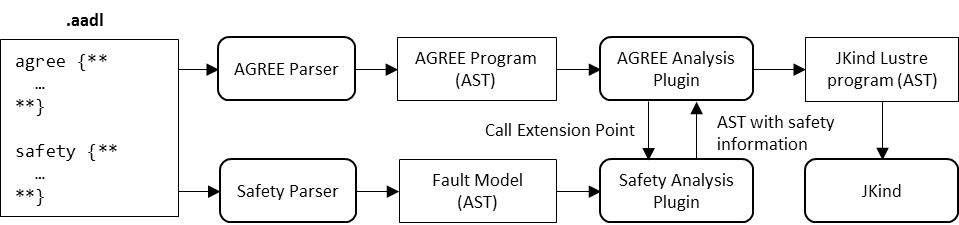
\includegraphics[trim=0 400 430 0,clip,width=0.85\textwidth]{images/arch.png}
		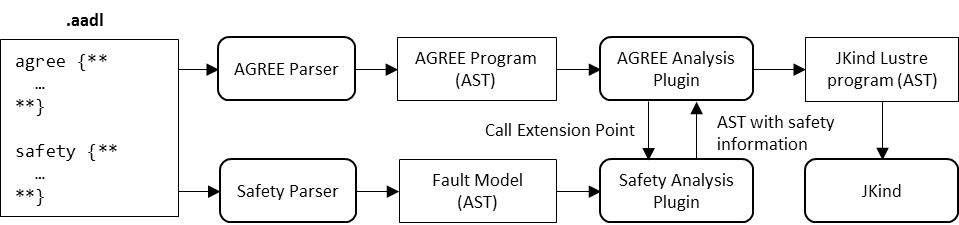
\includegraphics[width=.9\textwidth]{images/arch.png}
	\end{center}
	\vspace{-0.2in}
	\caption{Safety Annex Plug-in Architecture}
	\label{fig:plugin-arch}
	\vspace{-0.2in}
\end{figure}

%\end{comment}

AGREE contracts are used to define the nominal behaviors of system components as {\em guarantees} that hold when {\em assumptions} about the values the component's environment are met.  The Safety Annex extends these contracts to allow faults to modify the behavior of component inputs and outputs. 
% To support these extensions, AGREE implements an Eclipse extension point interface that allows other plug-ins to modify the generated abstract syntax tree (AST) prior to its submission to the solver.  If the Safety Annex is enabled, these faults are added to the AGREE contract and, when triggered, override the nominal guarantees provided by the component.  
An example of a portion of an initial AGREE node and its extended contract is shown in Figure~\ref{fig:lustre}. The left column of the figure shows the nominal Lustre pump definition is shown with an AGREE contract on the output; and the right column shows the additional local variables for the fault (boxes 1 and 2), the assertion binding the fault value to the nominal value (boxes 3 and 4), and the fault node definition (box 5).

%In the left column of the figure, the nominal Lustre pump definition is shown with an AGREE contract on the output. In the right column, the additional local variables for the fault are seen in boxes 1 and 2, the assertion binding the fault value to the nominal value is seen in boxes 3 and 4, and the fault node definition is given in box 5. 

Once augmented with fault information, the AGREE model follows the standard translation path to the model checker JKind~\cite{2017arXiv171201222G}, an infinite-state model checker for safety properties.  The augmentation includes traceability information so that when counterexamples are displayed to users, the active faults for each component are visualized.

\begin{figure}[h!]
	\hspace*{-2cm}
	\vspace{-0.3in} 
	\begin{center}
		%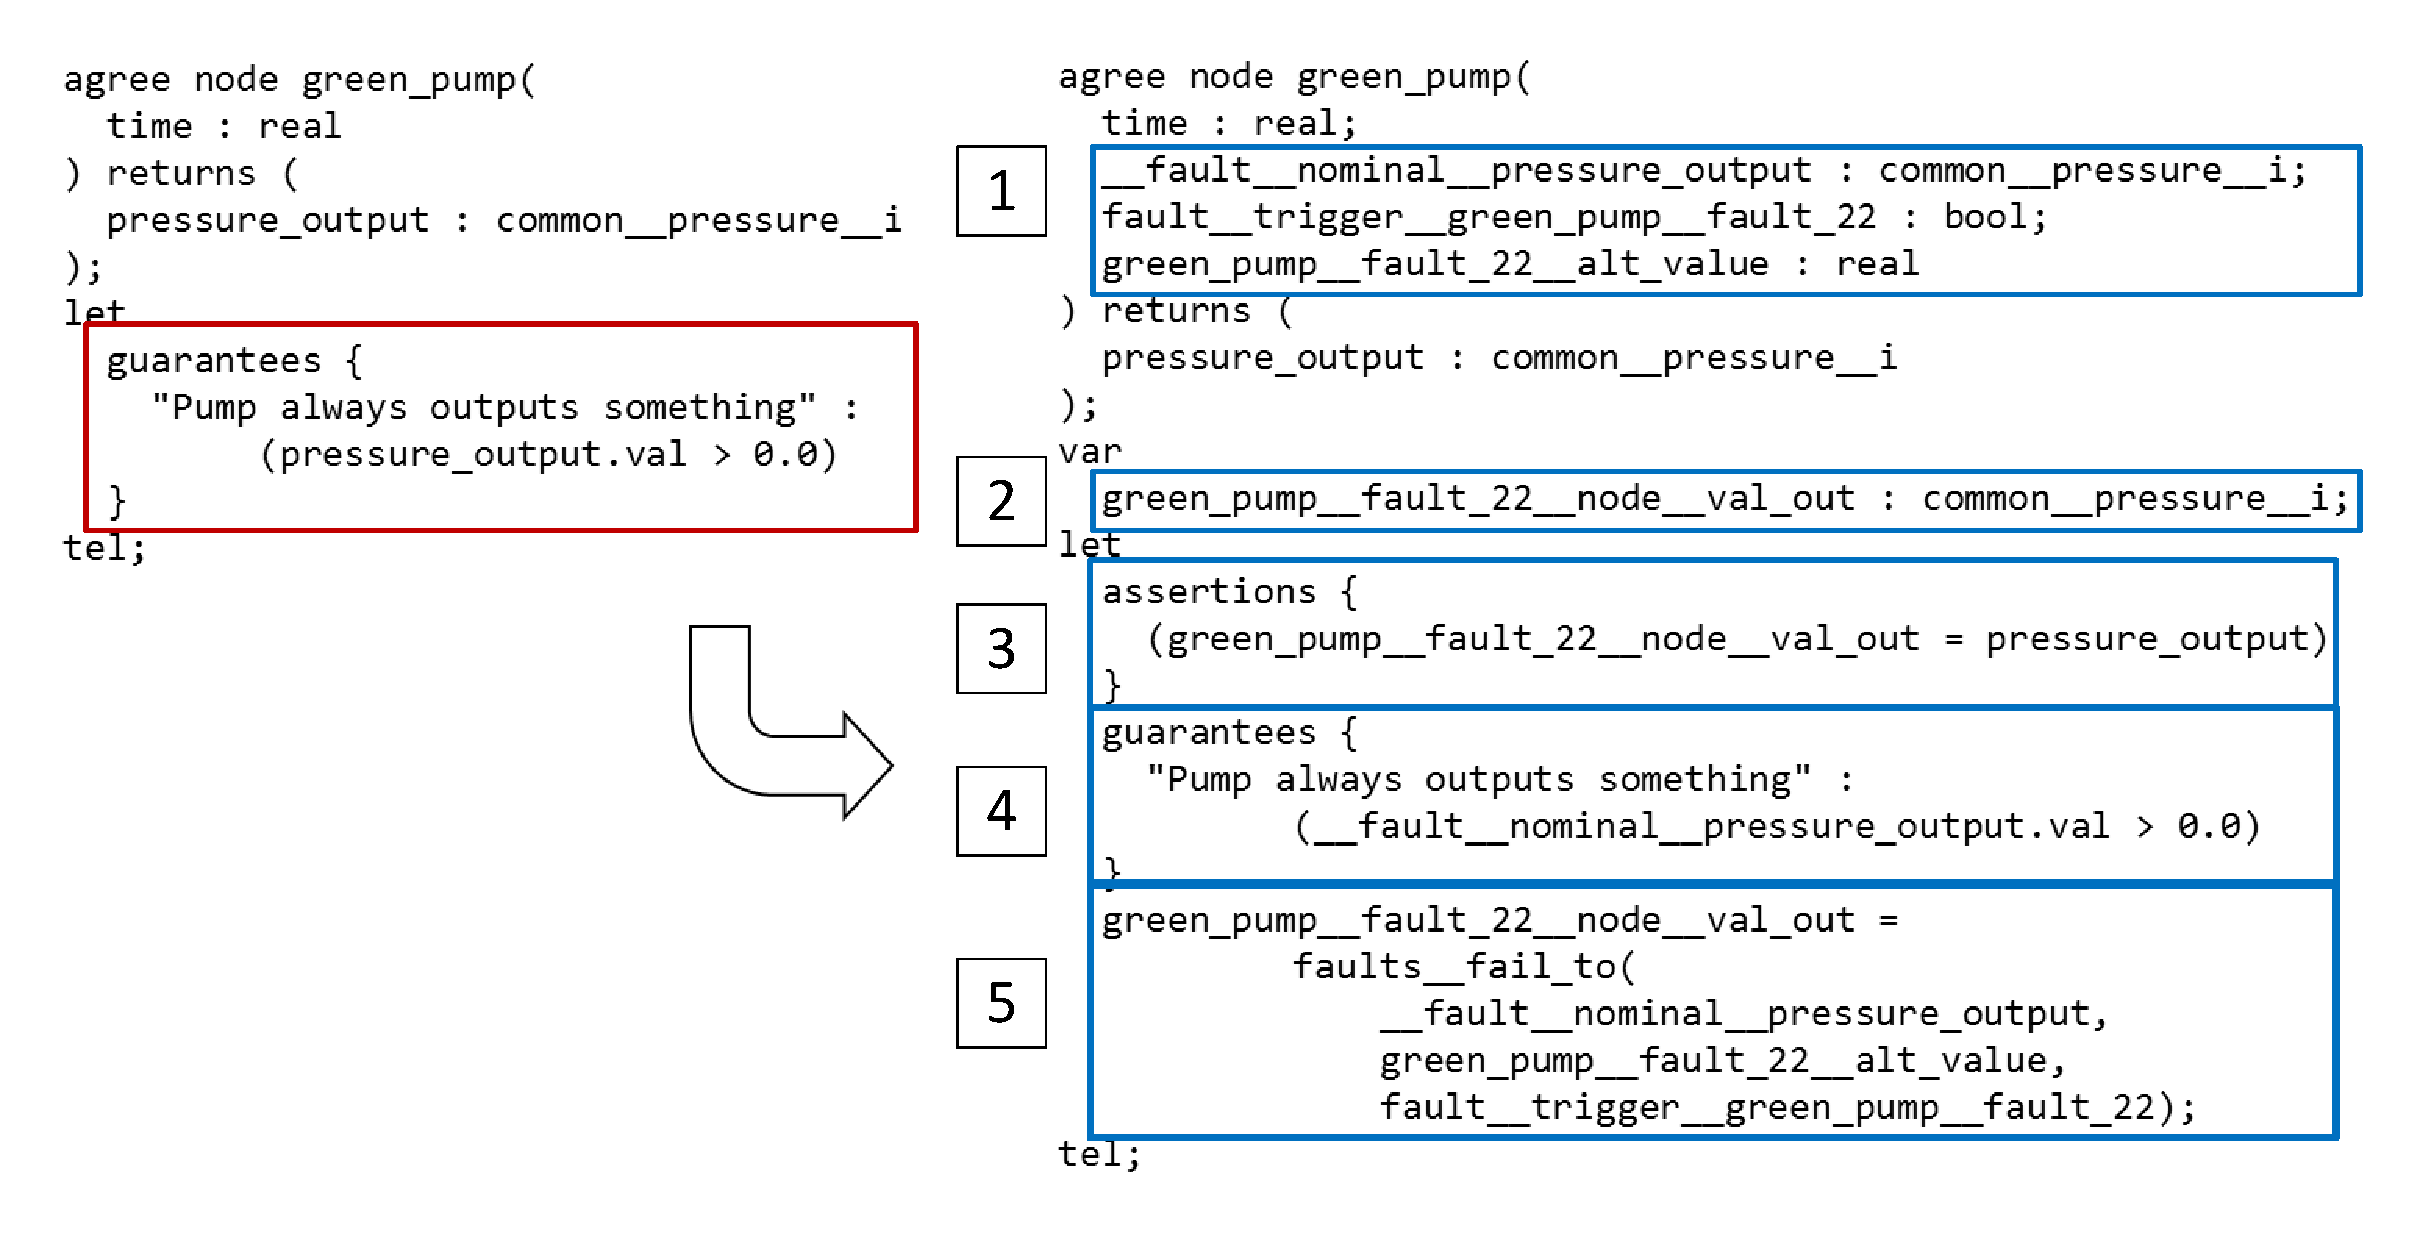
\includegraphics[trim=0 690 -10 70,clip,width=1.5\dimexpr\textwidth-2cm\relax]{images/lustre.pdf}
		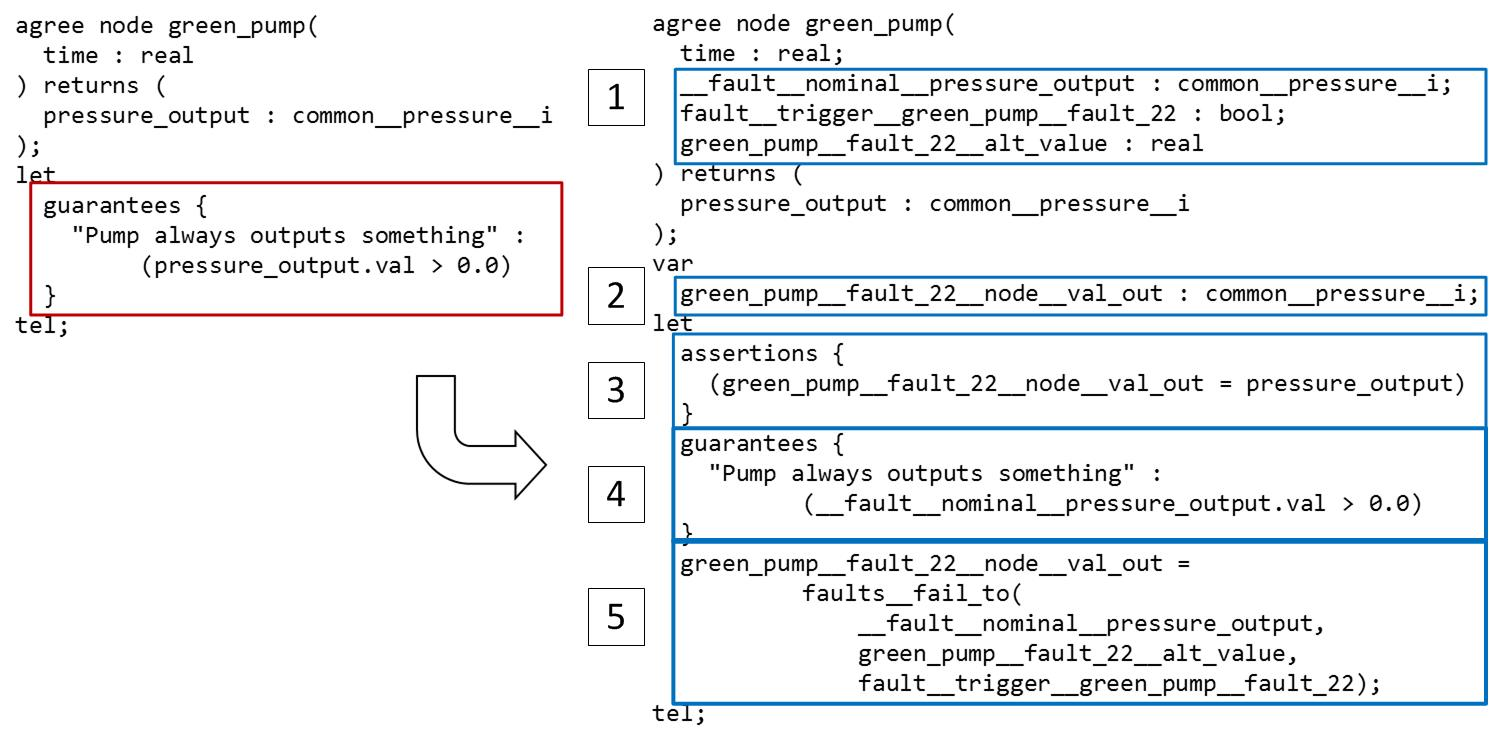
\includegraphics[scale=0.3]{images/lustre.jpg}
		%\caption{Nominal AGREE node and its extension with faults}
	\caption{Nominal AGREE Node and Extension with Faults}
		\label{fig:lustre}
	\end{center}
	\vspace{-0.3in}
\end{figure}

\begin{comment}
The architecture of the Safety Annex is shown in Figure~\ref{fig:plugin-arch}.  It is written in Java as a plug-in for the OSATE AADL toolset, which is built on Eclipse.  It is not designed as a stand-alone extension of the language, but works with behavioral contracts specified in AGREE AADL annex and associated tools~\cite{NFM2012:CoGaMiWhLaLu}.  AGREE allows {\em assume-guarantee} behavioral contracts to be added to AADL components.  The language used for contract specification is based on the Lustre dataflow language~\cite{Halbwachs91:IEEE}. AGREE improves scalability of formal verification to large systems by decomposing the analysis of a complex system architecture into a collection of smaller verification tasks that correspond to the structure of the architecture.

\begin{figure}
	\begin{center}
		%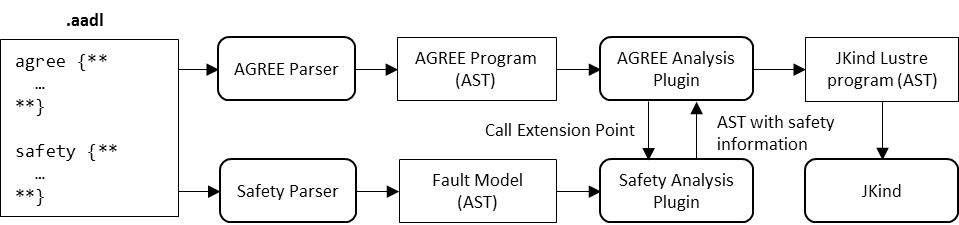
\includegraphics[trim=0 400 430 0,clip,width=0.85\textwidth]{images/arch.png}
		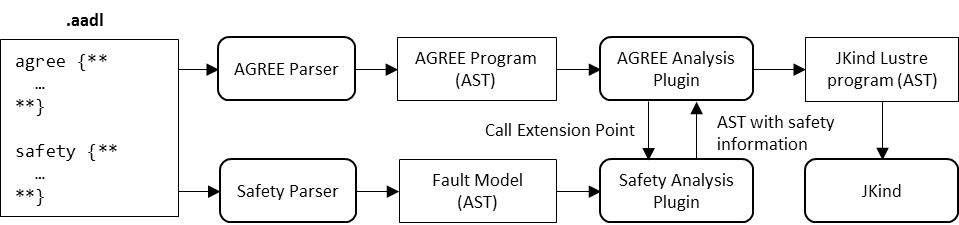
\includegraphics[width=.9\textwidth]{images/arch.png}
	\end{center}
	\vspace{-0.2in}
	\caption{Safety Annex Plug-in Architecture}
	\label{fig:plugin-arch}
\end{figure}

AGREE contracts are used to define the nominal behaviors of system components as {\em guarantees} that hold when {\em assumptions} about the values the component's environment are met.  The Safety Annex extends these contracts to allow faults to modify the behavior of component inputs and outputs.  To support these extensions, AGREE implements an Eclipse extension point interface that allows other plug-ins to modify the generated abstract syntax tree (AST) prior to its submission to the solver.  If the Safety Annex is enabled, these faults are added to the AGREE contract and, when triggered, override the nominal guarantees provided by the component.  

An example of a portion of an initial AGREE node and its extended contract is shown in Figure~\ref{fig:lustre}. 
In the left column of the figure, the nominal Lustre pump definition is shown with an AGREE contract on the output. In the right column, the additional local variables for the fault are seen in boxes 1 and 2, the assertion binding the fault value to the nominal value is seen in boxes 3 and 4, and the fault node definition is given in box 5. 

\begin{figure}[h!]
	\hspace*{-2cm}
	\vspace{-0.3in} 
	\begin{center}
		%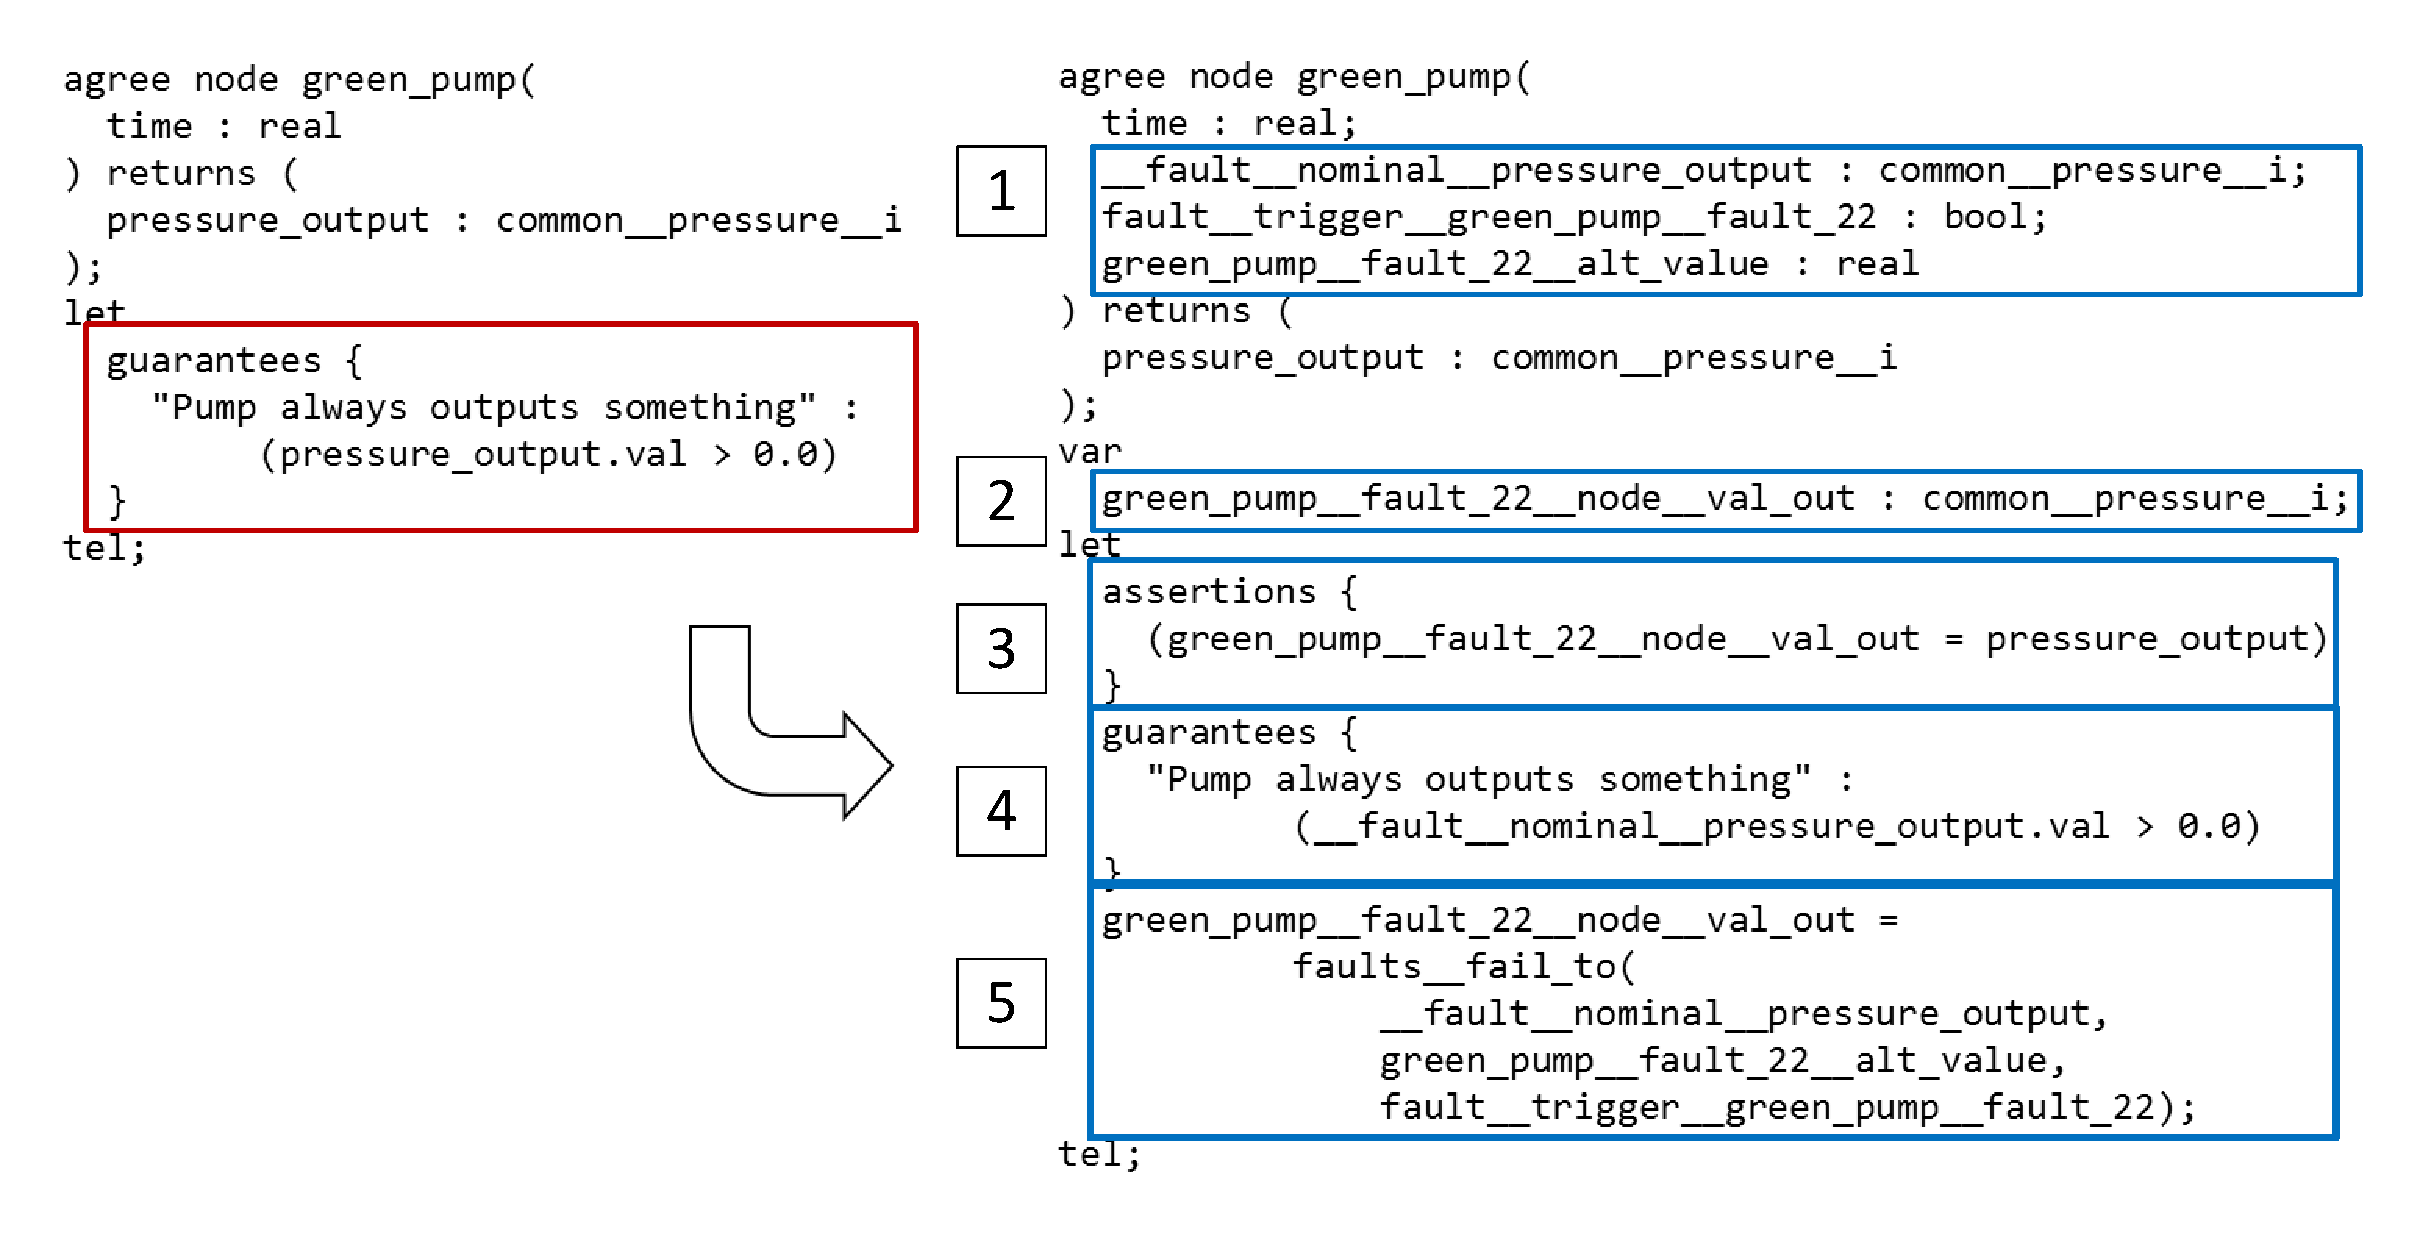
\includegraphics[trim=0 690 -10 70,clip,width=1.5\dimexpr\textwidth-2cm\relax]{images/lustre.pdf}
		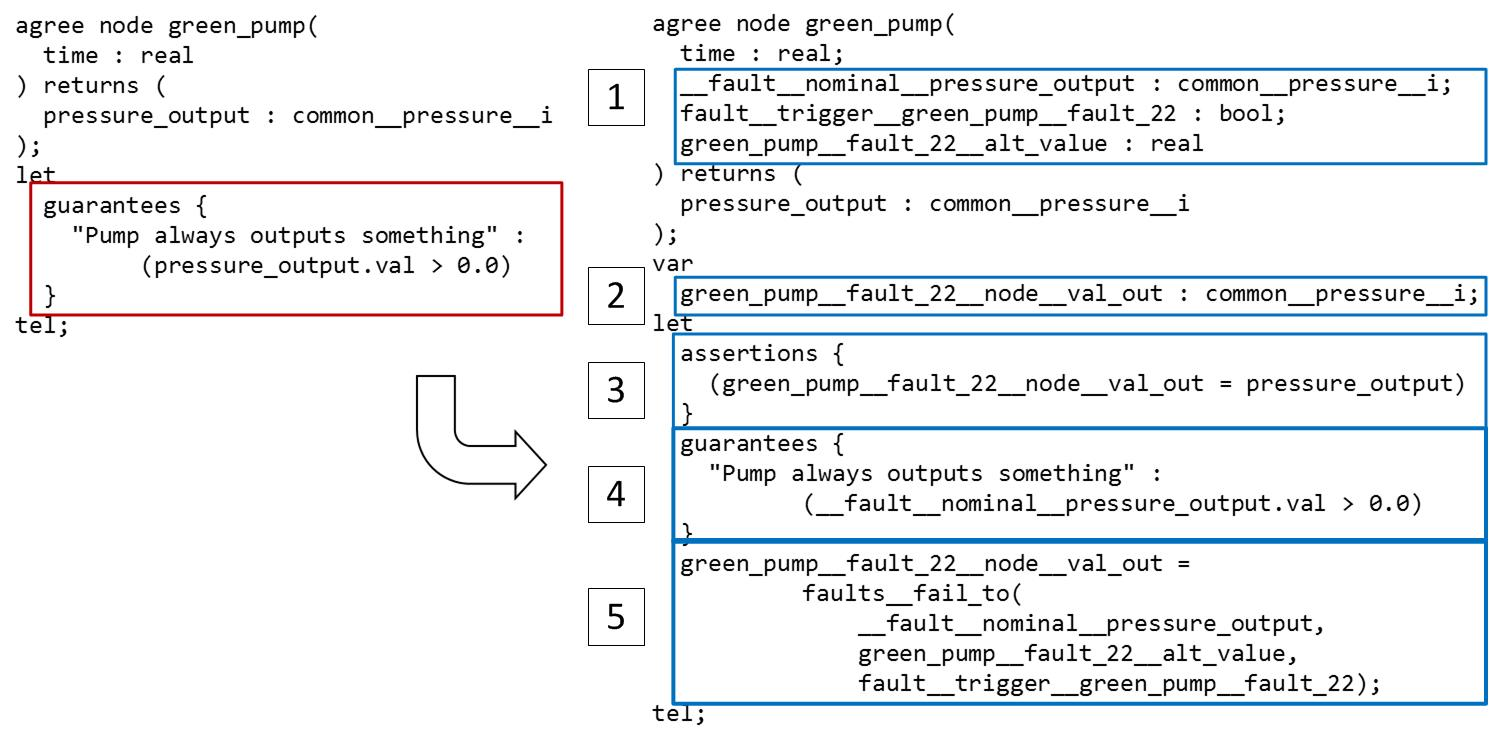
\includegraphics[scale=0.3]{images/lustre.jpg}
		\caption{Nominal AGREE node and its extension with faults}
		\label{fig:lustre}
	\end{center}
	\vspace{-0.3in}
\end{figure}


Once augmented with fault information, the AGREE model follows the standard translation path to the model checker JKind~\cite{2017arXiv171201222G}, an infinite-state model checker for safety properties.  The augmentation includes traceability information so that when counterexamples are displayed to users, the active faults for each component are visualized.

The architecture of the Safety Annex is shown in Figure~\ref{fig:plugin-arch}.  It is written in Java as a plug-in for the OSATE AADL toolset, which is built on Eclipse.  It is not designed as a stand-alone extension of the language, but works with behavioral contracts specified in AGREE AADL annex and associated tools~\cite{NFM2012:CoGaMiWhLaLu}.  AGREE allows {\em assume-guarantee} behavioral contracts to be added to AADL components.  The language used for contract specification is based on the Lustre dataflow language~\cite{Halbwachs91:IEEE}. AGREE improves scalability of formal verification to large systems by decomposing the analysis of a complex system architecture into a collection of smaller verification tasks that correspond to the structure of the architecture.

\begin{figure}
	\begin{center}
		%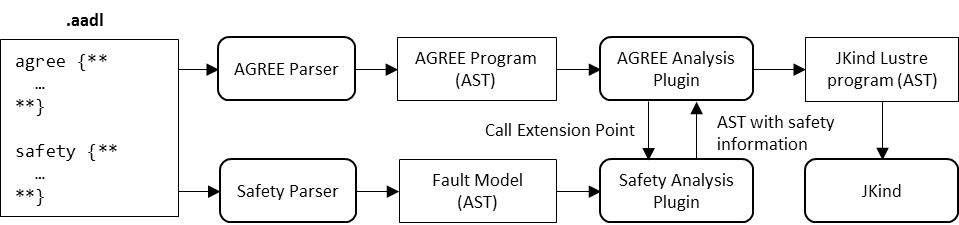
\includegraphics[trim=0 400 430 0,clip,width=0.85\textwidth]{images/arch.png}
		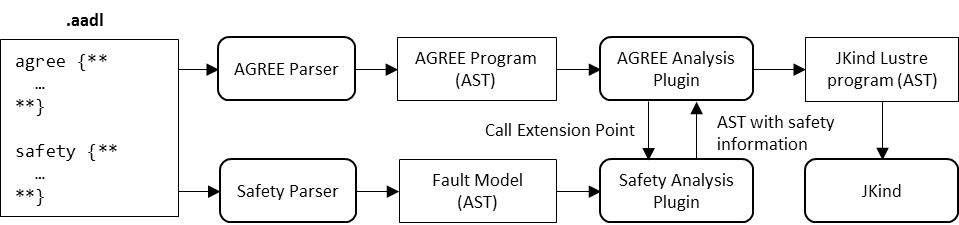
\includegraphics[width=.9\textwidth]{images/arch.png}
	\end{center}
	\vspace{-0.2in}
	\caption{Safety Annex Plug-in Architecture}
	\label{fig:plugin-arch}
\end{figure}

AGREE contracts are used to define the nominal behaviors of system components as {\em guarantees} that hold when {\em assumptions} about the values the component's environment are met.  The Safety Annex extends these contracts to allow faults to modify the behavior of component inputs and outputs.  To support these extensions, AGREE implements an Eclipse extension point interface that allows other plug-ins to modify the generated abstract syntax tree (AST) prior to its submission to the solver.  If the Safety Annex is enabled, these faults are added to the AGREE contract and, when triggered, override the nominal guarantees provided by the component.  

An example of a portion of an initial AGREE node and its extended contract is shown in Figure~\ref{fig:lustre}.  %The \texttt{\_\_fault} variables and declarations are added to allow the contract to override the nominal behavioral constraints (provided by guarantees) on outputs.  In the Lustre language, \texttt{assertion}s are constraints that are assumed to hold in the transition system. 
In the left column of the figure, the nominal Lustre pump definition is shown with an AGREE contract on the output. In the right column, the additional local variables for the fault are seen in boxes 1 and 2, the assertion binding the fault value to the nominal value is seen in boxes 3 and 4, and the fault node definition is given in box 5. 

%A  benefit of utilizing the AGREE behavioral annex is the ability to perform both monolithic and compositional analysis on the nominal model. AGREE allows {\em assume-guarantee} behavioral contracts to be added to AADL components.  The language used for contract specification is based on the Lustre dataflow language~\cite{Halbwachs91:IEEE} and the nominal model (AADL model annotated with AGREE contracts) is translated into Lustre before being sent to the JKind model checker for verification\cite{2017arXiv171201222G}. 

%When a user selects to run the fault analysis during verification, the AGREE contracts are automatically extended in Lustre in order to allow faults to modify the behavior of component outputs. These injections into the Lustre model are shown in Figure~\ref{fig:lustre}. 

\begin{figure}[h!]
	\hspace*{-2cm}
	\vspace{-0.3in} 
	\begin{center}
		%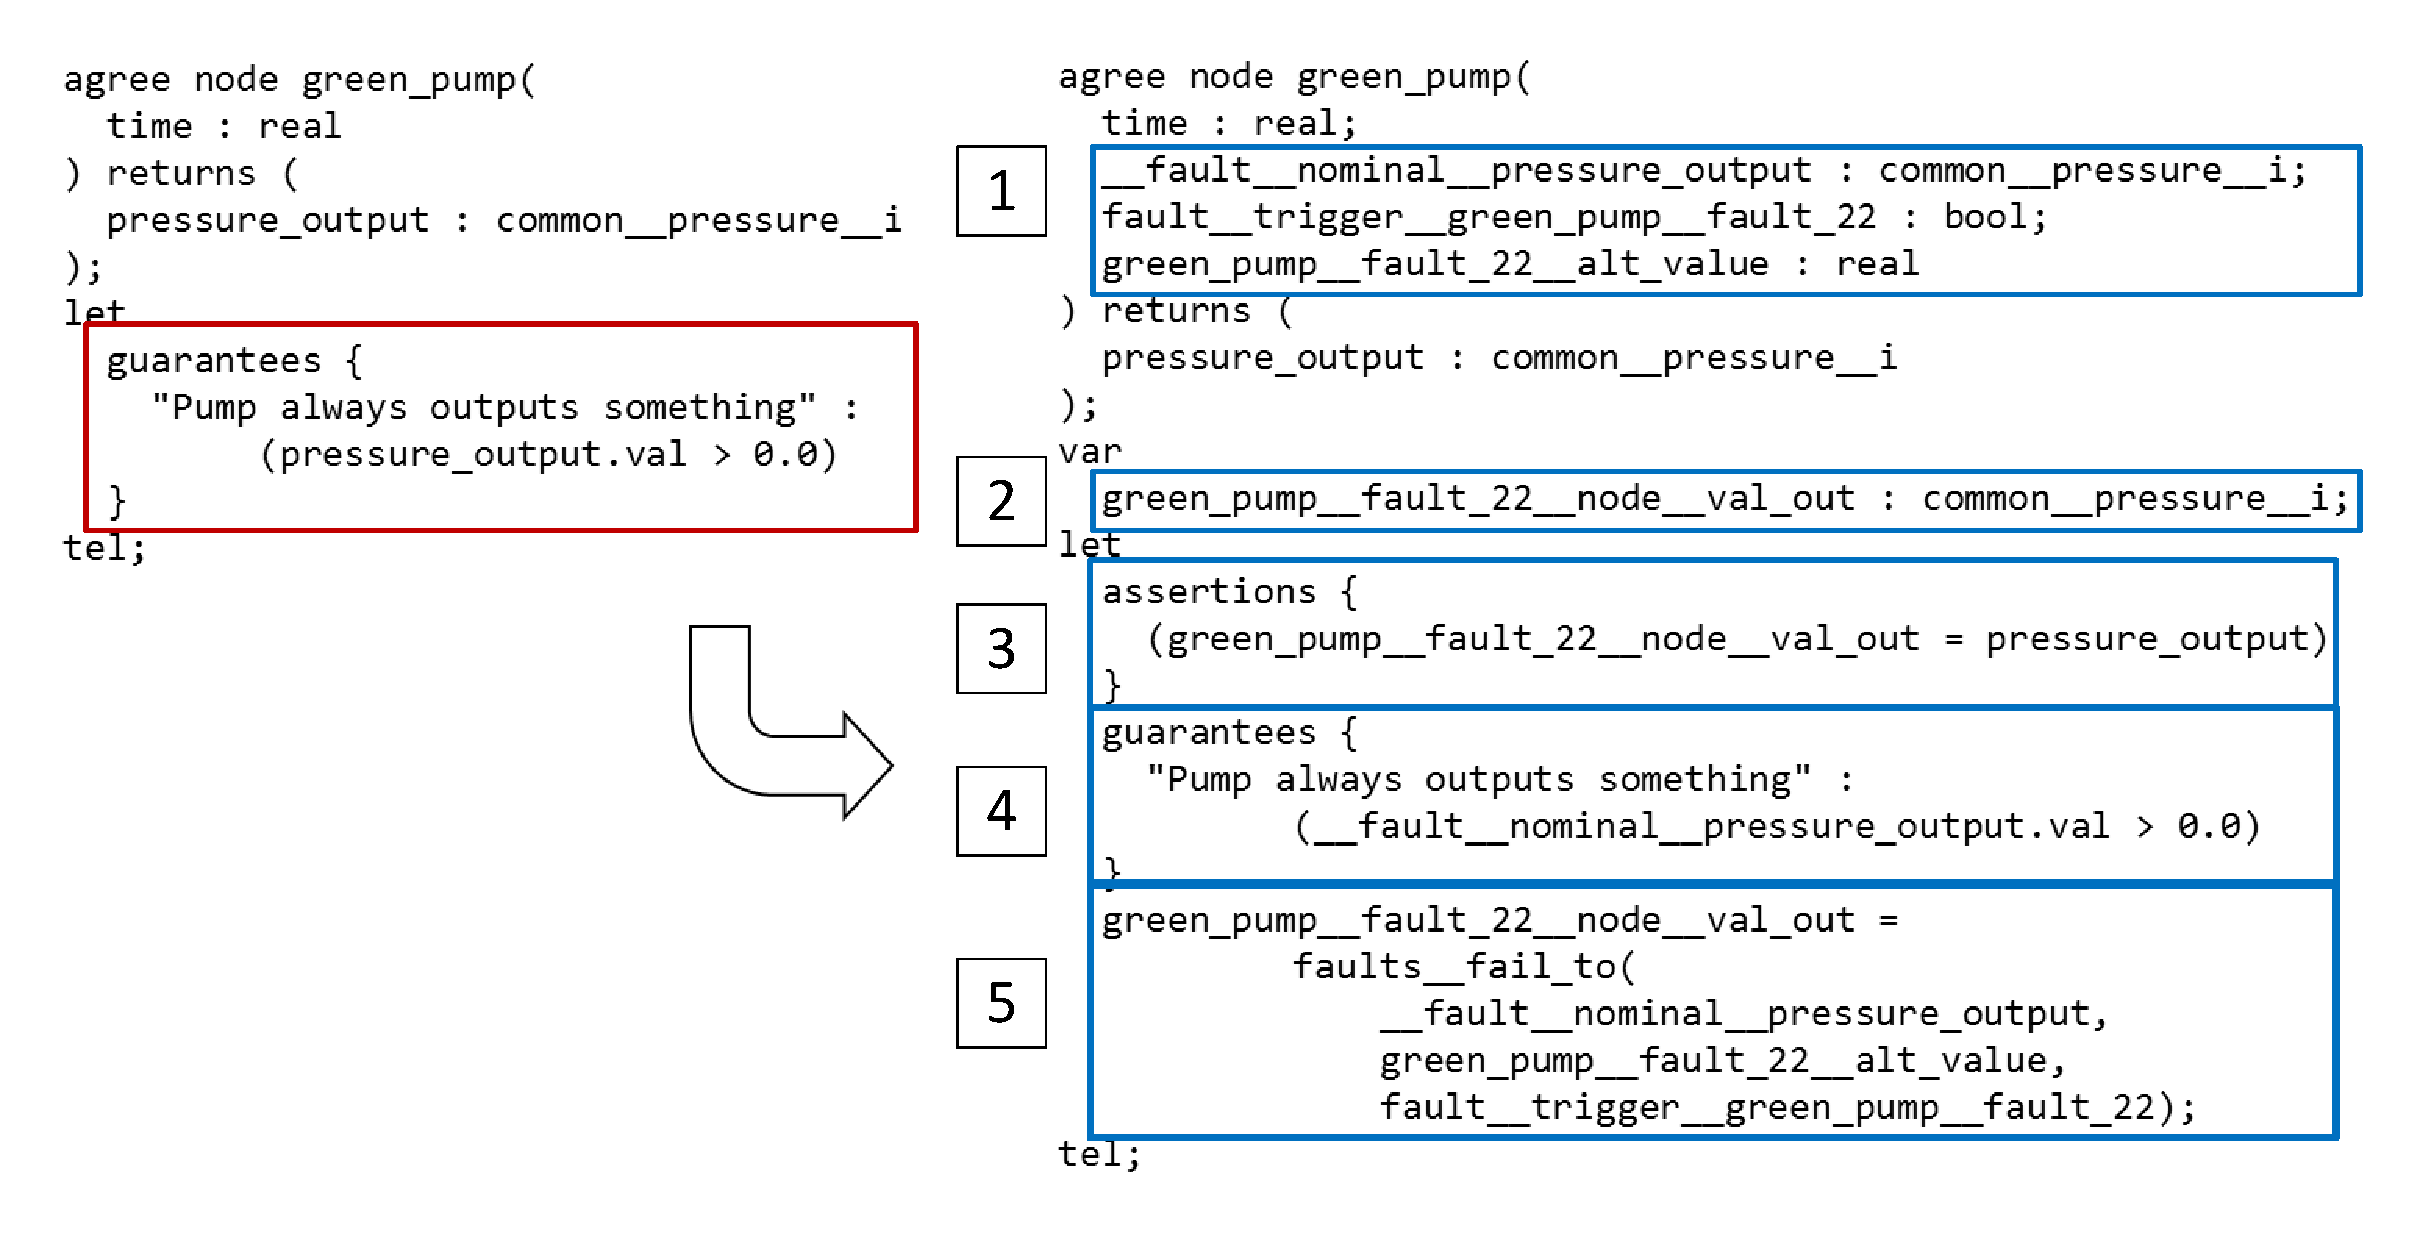
\includegraphics[trim=0 690 -10 70,clip,width=1.5\dimexpr\textwidth-2cm\relax]{images/lustre.pdf}
		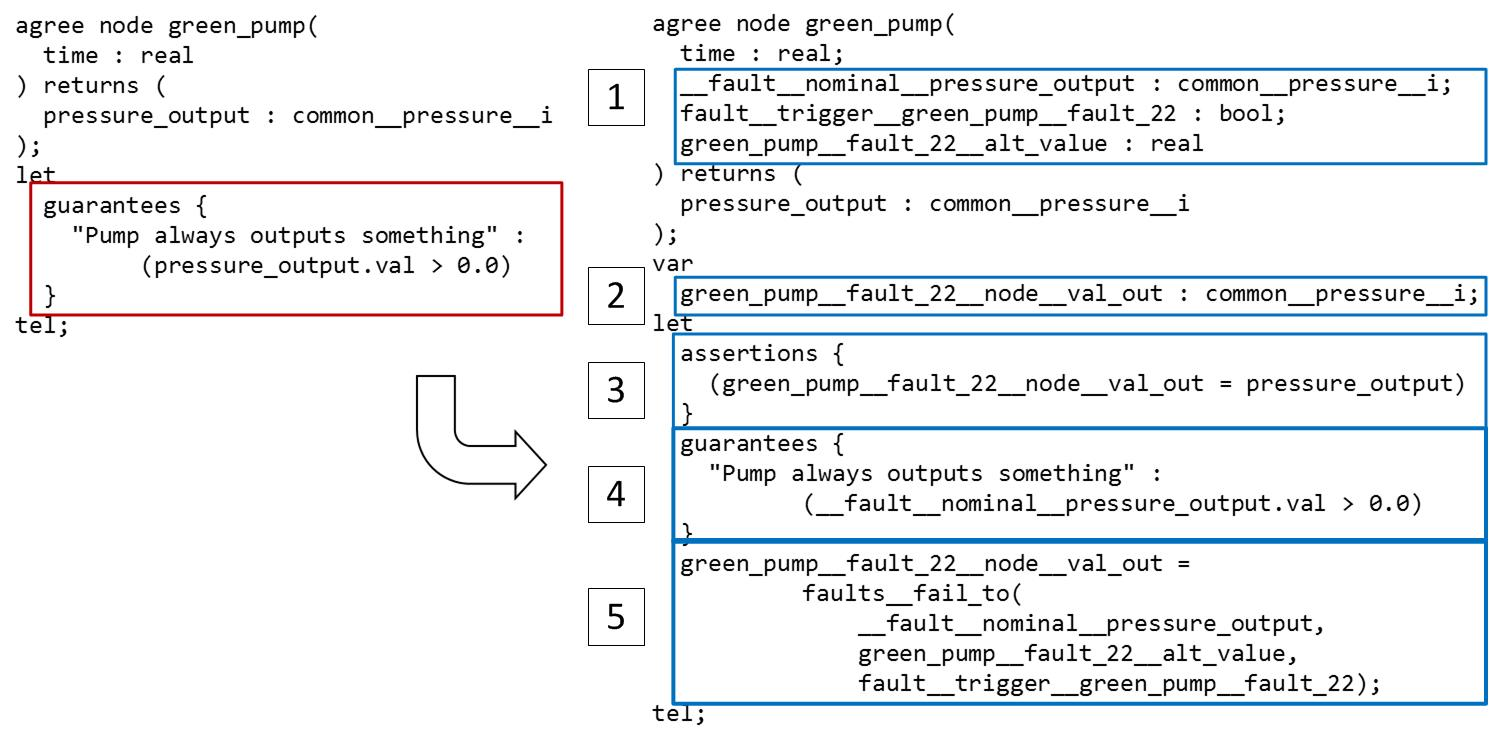
\includegraphics[scale=0.3]{images/lustre.jpg}
		\caption{Nominal AGREE node and its extension with faults}
		\label{fig:lustre}
	\end{center}
	\vspace{-0.3in}
\end{figure}

\begin{comment}
\begin{figure}
	\vspace{-0.1in}
	%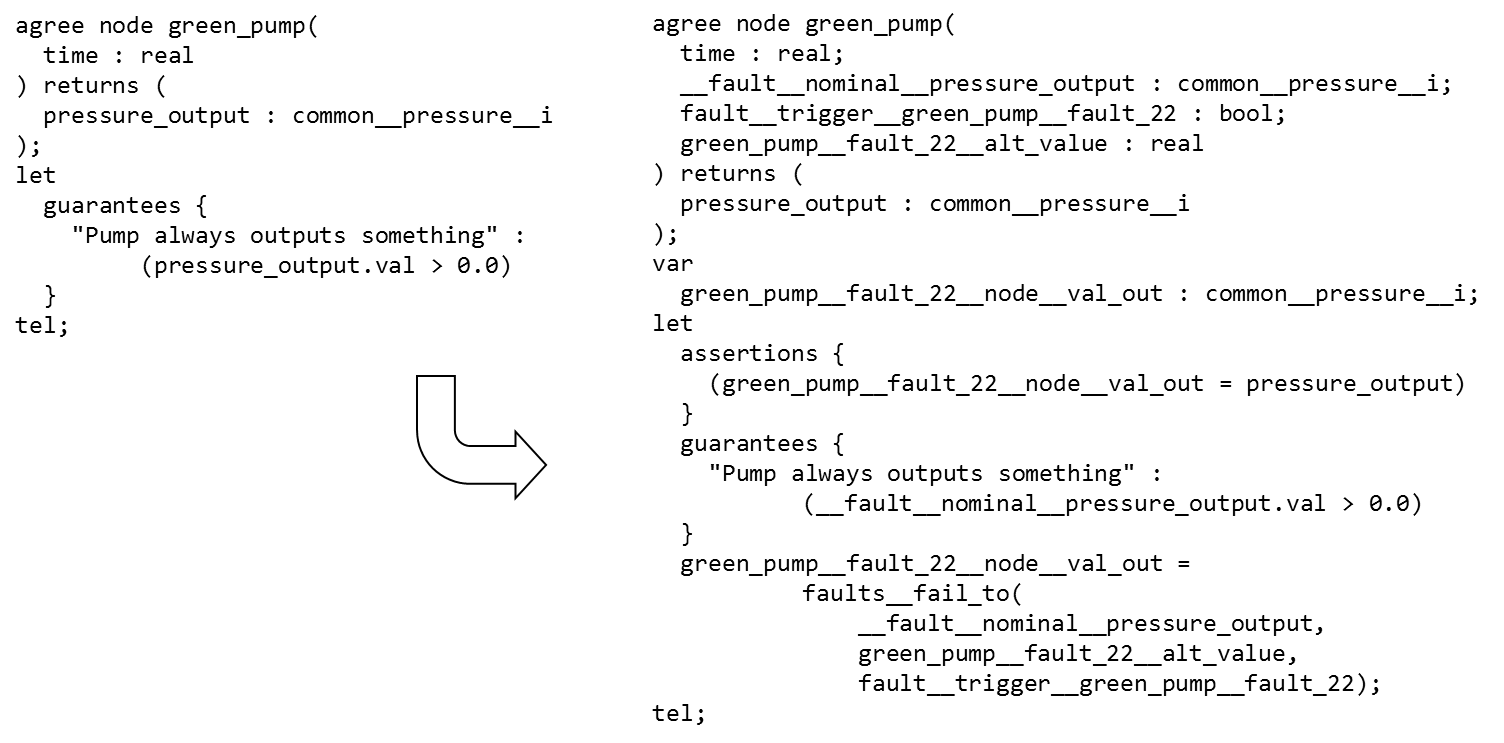
\includegraphics[trim=30 150 120 10,clip,width=\textwidth]{images/sample_code.png}
	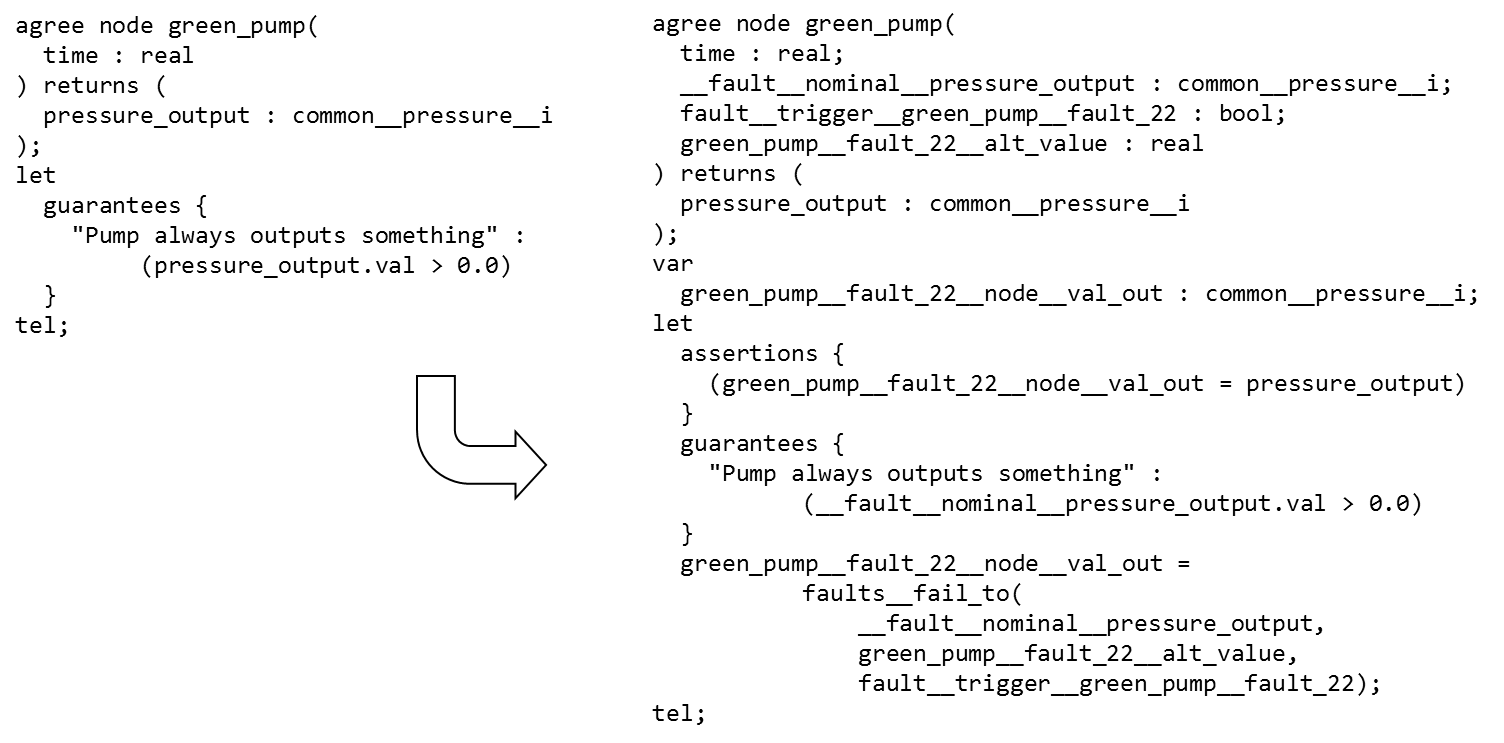
\includegraphics[width=\textwidth]{images/sample_code.png}
	\vspace{-0.3in}
	\caption{Nominal AGREE node and its extension with faults}
	\label{fig:comp}
\end{figure}
\end{comment}
%An annotation in the AADL model determines the fault hypothesis.  This may specify either a maximum number of faults that can be active at any point in execution (typically one or two), or that only faults whose probability of simultaneous occurrence is above some probability threshold should be considered. In the former case, we assert that the sum of the true {\em fault\_\_trigger} variables is below some integer threshold.  In the latter, we determine all combinations of faults whose probabilities are above the specified probability threshold, and describe this as a proposition over {\em fault\_\_trigger} variables.
%
%With the introduction of dependent faults, active faults are divided into two categories: independently active (activated by its own triggering event) and dependently active (activated when the faults they depend on become active). The top level fault hypothesis applies to independently active faults. Faulty behaviors augment nominal behaviors whenever their corresponding faults are active (either independently active or dependently active).

%Once augmented with fault information, the AGREE model follows the standard translation path to the model checker JKind~\cite{2017arXiv171201222G}, an infinite-state model checker for safety properties.  The augmentation includes traceability information so that when counterexamples are displayed to users, the active faults for each component are visualized.


%For fault analysis, we separate the possible analyses available to users into two distinct actions and describe them here.


\section{Analysis of the Fault Model}
\label{sec:fault_analysis}

When the Safety Annex is enabled, users can invoke either the monolithic analysis or compositional analysis in AGREE to check if the top level safety properties of the system hold in the presence of faults under the fault hypothesis given for the system. If an active fault causes the violation of a contract, a counterexample is provided by the model checker. The counterexample can be used to further analyze the system design and make necessary updates to the shared model between safety assessment and system development processes. This iterations continues until the system safety property is satisfied with the desired fault tolerance and failure probability achieved.

\subsection{Fault Hypothesis}
As the number of component faults increases, the different fault combinations can grow exponentially, making model checking infeasible. Therefore, a fault hypothesis needs to be specified for the system under verification to limit the simultaneous fault activations that are considered by the model checker.

A Safety Annex annotation in the system implementation of the AADL model determines the fault hypothesis. There are two types of fault hypothesis:

The \textit{max fault hypothesis} specifies a maximum number of faults that can be active at any point in execution. This is analogous to restricting the cutsets to a specified maximum number of terms in the fault tree analysis in
traditional safety analysis. In implementation (i.e., the translated Lustre model feeding into the model checker), we assert that the sum of the true {\em fault\_\_trigger} variables is below some integer threshold. Each layer of the model needs to have a max fault hypothesis statement specified in order to consider fault activation in that layer in the analysis.

The \textit{probabilistic fault hypothesis} specifies that only faults whose probability of simultaneous occurrence is above some probability threshold should be considered. This is analogous to restricting the cutsets to only those whose probability is above some set value. In implementation, we determine all combinations of faults whose probabilities are above the specified probability threshold and describe this as a proposition over {\em fault\_\_trigger} variables. Each subcomponent fault needs to specify a probability of occurrence in order to be considered in the analysis.

With the introduction of dependent faults, active faults are divided into two categories: independently active (activated by its own triggering event) and dependently active (activated when the faults they depend on become active). The top level fault hypothesis applies to independently active faults. Faulty behaviors augment nominal behaviors whenever their corresponding faults are active (either independently active or dependently active).

\subsection{Monolithic Analysis}
When monolithic analysis is performed on the nominal system model, the architectural model is flattened in order to perform the analysis. All of the contracts in the lower levels are used for the analysis.

Given a probabilistic fault hypothesis, this corresponds to performing a %prior 
analysis on which combinations of faults have a probability less than the threshold and then inserting assertions into the Lustre code accordingly. If the probability of such combination of faults is in fact less than the designated top level threshold, these faults may be activated and the behavioral effects can be seen through a counterexample.  

To perform this analysis, it is assumed that the non-hardware faults occur independently and possible combinations of faults are computed and passed to the Lustre model to be checked by the model checker. As seen in Algorithm 1, the computation first removes all faults from consideration that are too unlikely given the probability threshold. The remaining faults are arranged in a priority queue $\mathcal{Q}$ from high to low. Assuming independence in the set of faults, we take a fault with highest probability from the queue (step 5) and attempt to combine the remainder of the faults in $\mathcal{R}$ (step 7). If this combination is lower than the threshold (step 8), then we do not take into consideration this set of faults and instead remove the tail of the remaining faults in $\mathcal{R}$. The reason we can do this is because of the arrangement in priority queue from highest to lowest value. If this combination is below threshold, certainly any other combination of these faults with one of lesser value in the priority queue will also be below threshold. 
 
In this calculation, we assume independence among the faults, but in the Safety Annex it is possible to define dependence between faults using a 
fault propagation statement. After fault combinations are computed using Algorithm 1, the triggered dependent HW faults are added to the combination as appropriate. 

\begin{algorithm}[H]
	% \KwData{this text}
	% \KwResult{how to write algorithm with \LaTeX2e }
	$\mathcal{F} = \{\}$ : fault combinations above threshold \;
	$\mathcal{Q}$ : faults, $q_i$, arranged with probability high to low \;
	$\mathcal{R} = \mathcal{Q}$ , with $r \in \mathcal{R}$\;
	\While{$\mathcal{Q} \neq \{\} \land \mathcal{R} \neq \{\}$ }{
		$q =$ removePriorityElement($\mathcal{Q}$) \;
		\For{$i=0:|\mathcal{R}|$}{
			$prob = q \times r_i$ \;
			\eIf{prob $<$ threshold}{
				removeTail($\mathcal{R}, j=i:|\mathcal{R}|$)\;
			}{
				add($\{q, r_i\}, \mathcal{Q}$)\;
				add($\{q, r_i\}, \mathcal{F}$)\;
			} % end if else
		} % end for
	} % end while
	\caption{Monolithic Probability Analysis}
\end{algorithm}

After all possible fault combinations are computed from Algorithm 1, we look at the collection of propagation statements used in HW fault definitions and add additional faults into the possible fault combinations if a fault that triggers the fault can become active, as computed from Algorithm 1.

At the end of Algorithm 1, the possible fault combinations reside in the list $\mathcal{F}$. We then look at the collection of propagation statements used in HW fault definitions. These have a source (HW fault) and destination (faults triggered by HW fault). 

Let $\mathcal{P}$ be the collection of propagation statements. For all $S \subset \mathcal{F}$, check to see if for $f \in S$, $f \in \mathcal{P}$ as a source. If so, add the corresponding destinations to the set $S$. This set $\mathcal{F}$ of allowed fault combinations is then added as a constraint to the Lustre model and thus they become active. If an active fault causes the violation of a contract, this is seen in a counterexample provided by the model checker.

\subsection{Compositional Analysis}
In compositional analysis, the analysis proceeds in a top down fashion. To prove the top level properties, the properties in the layer directly beneath the top level are used to perform the proof. The analysis proceeds in this manner.

The compositional analysis currently works with the max fault hypothesis. Users can constrain the maximum number of faults within each layer of the model by specifying the maximum fault hypothesis statement to that layer. If any lower level property failed due to activation of faults, the property verification at the higher level can no longer be trusted because the higher level properties were proved based on the assumption that the direct sublevel contracts are valid.

The compositional analysis is helpful to see weaknesses in a given 
layer of the system. In future work, we plan to reflect lower layer
property violations in the verification results of higher layers in the architecture and enable the display or constraint active faults system wide instead of layer wide.



\section{Related Work}
\label{sec:related_work}
Minimal cut sets generated by monolithic analysis look only at explicitly defined faults throughout the architecture and attempt through various techniques to find the minimal violating set for a particular property. We outline some of the common monolithic approaches to minimal cut set generation in this section.

The representation of Boolean formulae as Binary Decision Diagrams (BDDs) was first formalized in the mid 1980s~\cite{bryant1986graph} and were extended to the representation of fault trees not many years later~\cite{rauzy1993new}. After this formalization, the BDD approach to FTA provided a new approach to safety analysis. The model is constructed using a BDD, then a second BDD - usually slightly restructured - is used to encode MinCutSets~\cite{rauzy2008binary}. Unfortunately, due to the structure of BDDs, the worst case is exponential in size in terms of the number of variables~\cite{bryant1986graph,rauzy1993new,rauzy2008binary}. In industrial sized systems, this is not realistically useful. 

SAT based computation was then introduced to address scalability problems in the BDD approach; initially it was used as a preprocessing step to simplify the decision diagram~\cite{bozzano2015safety}, but later extended to allow for all MinCutSet processing and generation without the use of BDDs~\cite{bozzano2015efficient}. Since then, numerous safety related research groups have focused on leveraging the power of model checking in the problems of safety assessment~\cite{bieber2002combination,schafer2003combining,bozzano2007symbolic,bozzano2003improving,volk2017fast,Joshi05:SafeComp,bozzano2015efficient,stewart2020safety}. 

Bozzano et al. formulated a Bounded Model Checking (BMC) approach to the problem by successively approximating the cut set generation and computations to allow for an ``anytime approximation" in cases when the cut sets were simply too large and numerous to find~\cite{bozzano2015efficient,mattarei2016scalable}. These algorithms are implemented in xSAP~\cite{DBLP:conf/tacas/BittnerBCCGGMMZ16} and COMPASS~\cite{compass30toolset}. 

The model based safety assessment tool AltaRica 3.0~\cite{prosvirnova:tel-01119730} performs a series of processing to transform the model into a reachability graph and then compile to Boolean formula in order to compute the MinCutSets~\cite{prosvirnova2015automated}. Other tools such as HiP-HOPS~\cite{papadopoulos2001model} have implemented algorithms that follow the failure propagations in the model and collect information about safety related dependencies and hazards. The Safety Analysis Modeling Language (SAML)~\cite{Gudemann:2010:FQQ:1909626.1909813} provides a safety specific modeling language that can be translated into a number of input languages for model checkers in order to provide model checking support for MinCutSet generation.

To our knowledge, a fully compositional approach to calculating minimal cut sets has not been introduced.





















\section{Conclusion}

An extension to the AADL language has been developed with tool support for formal analysis of system safety properties in the presence of faults. Faulty behavior is specified as an extension of the nominal model, allowing safety analysis and system implementation to be driven from a single common model. This new Safety Annex leverages the AADL structural model and nominal behavioral specification (using the AGREE annex) to propagate faulty component behaviors without the need to add separate propagation specifications to the model.   Next steps will include extensions to automate injection of Byzantine faults as well as automatic generation of fault trees.  For more details on the tool, models, and approach, see the technical report and the repository~\cite{SATechReport, amaseRepo}.

\vspace{2 mm}
\noindent {\bf Acknowledgments.} This research was funded by NASA contract NNL16AB07T and the University of Minnesota College of Science and Engineering Graduate Fellowship.




\vspace{-0.40cm}
\bibliographystyle{abbrv}
\bibliography{biblio}
%\vspace{-7.25cm}
% This ~ seems to fix an odd bibliography alignment issue
~

%\ifdefined\TECHREPORT
%\appendix
%
%\section{Appendix: Proof of Equivalence}
%\input{appendix}
%\fi

%\section{Appendix: GPCA CENTA Model}
%\label{appendix:gpcacenta}
%\begin{figure}[!ht]
%\begin{center}
%\includegraphics[scale=0.6]{images/sampled_pca.PNG} %[trim = 0 2 0 0, clip=true]{Comp}
%\caption{GPCA AGREE Properties modeled as a Timed Automata} \label{fig:samplepca}
%\end{center}
%\end{figure}

%\balancecolumns

\end{document} 